\documentclass[11pt]{report}
\usepackage[
  proposal
 % ,final
 ,raggedbottom
%,tocbold        % uncomment to enable bold chapter titles in the ToC
                 %
                 % the style guidelines state that page numbers in the
                 % ToC should not be bold, but leave it up to the author
                 % and specific department guidelines as to how the
                 % chapter (or other section) titles should be typeset.
]{USCthesis}

% guidelines for manuscript formatting: https://graduateschool.usc.edu/wp-content/uploads/2020/11/Manuscript_Formatting_and_Documentation_Styles.pdf

%% our customizations %%%%%%%%%%%%%%%%%%%%%%%%%%%%%%%%%%%%%%%%%%%%%%%%%%
\usepackage[export]{adjustbox} % for frame option in \includegraphics
\usepackage{amsmath}
\usepackage{amssymb}
\usepackage{mathtools}
\usepackage{array}
\usepackage[utf8]{inputenc} % load inputenc before csquotes
\usepackage[english]{babel}
% \usepackage[
%   backend     = biber,
%   doi         = true,
%   hyperref    = true,
%   maxbibnames = 99,
%   sortlocale  = en_US,
%   style       = numeric,
% ]{biblatex}
\usepackage[authordate, backend=biber, autocite=inline]{biblatex-chicago}

\usepackage{booktabs}
\usepackage{color, colortbl}
\usepackage{csquotes}
\usepackage{efbox}
\usepackage{enumitem}
\usepackage[shortcuts]{extdash} % use `\-/' to hyphenate words/phrases that have a dash in them
\usepackage[tt=false]{libertine} % libertine's \ttfamily isn't that great
\usepackage[T1]{fontenc} % load fonts before fontenc
\usepackage[symbol]{footmisc}
\usepackage[
  showframe = false,% draw a border around textwidth
  pass      = true, % force 8.5"x11" pagesize
]{geometry}
\usepackage{graphicx}
%\usepackage[notquote]{hanging} % enables negative indents in paragraphs
\usepackage{hyphenat}
\usepackage{ifthen}
\usepackage{lipsum}
\usepackage{multirow}
\usepackage{parnotes}
\usepackage{pdflscape} % rotate some pages in an {landscape} environment
\usepackage{pifont}
\usepackage{ragged2e}
\usepackage{seqsplit}
\usepackage{siunitx}
\usepackage{subcaption}
\usepackage{tabularx}
\usepackage{xcolor}
\usepackage{xspace}
\usepackage{url}

% \usepackage[
%   breaklinks    = false,
%   colorlinks    = false,
%   hypertexnames = false,
%   pdfpagelabels = false,
%   citecolor     = {blue!80!black},
%   linkcolor     = {blue!80!black},
%   urlcolor      = {blue!80!black}
% ]{hyperref} % load hyperref as the last package

% pkg: biblatex
\setlength\bibitemsep{0.5\baselineskip}                 % add a line between entries
\AtEveryBibitem{\iffieldundef{doi}{}{\clearfield{url}}} % if DOI, hide URL

\addbibresource{references.bib}

% pkg: siunitx
% some guidelines https://physics.nist.gov/cuu/Units/checklist.html
\sisetup{
  tight-spacing  = true
  ,detect-family = true
  ,detect-mode   = true
  ,binary-units  = true    % support for MB, GB, etc.
  ,range-units   = single  % "3% to 5%" -> "3 to 5%"
  ,range-phrase  = --      % "3 to 5%"  -> "3--5%"
}

% pkg: babel, hyperref
% \addto\extrasenglish{%
%   \renewcommand{\chapterautorefname}{Chapter}
%   \renewcommand{\sectionautorefname}{Section}
%   \renewcommand{\subsectionautorefname}{Section}
%   \renewcommand{\subsubsectionautorefname}{Section}
% }

% pkg: url
\renewcommand{\UrlFont}{\footnotesize\tt}

% our custom commands
\renewcommand{\ttdefault}{cmtt} % use computer modern for teletype

%%% draft mode / toggle commands %%%
\usepackage{etoolbox}
\newtoggle{draft}
\settoggle{draft}{true} % change toggle for draft or final versions

\iftoggle{draft}{
  % if 'draft' toggle is true
  \overfullrule=10pt                       % highlight overfull hboxes
}{
  % if 'draft' toggle is false
  \PassOptionsToPackage{final}{showlabels} % hide labels on figures, etc
}

% if you're including existing papers into your thesis, it helps to put
% content behind a toggle (or conditional) so you only have to maintain
% and keep consistency on one copy. see "introduction.tex".
\newtoggle{thesis}
\settoggle{thesis}{false}
% \proposaltrue
% \newtoggle{proposal} %!!! Jeff
% \settoggle{proposal}{true}

% \usepackage[inline]{showlabels} # labels in blue!
% \renewcommand{\showlabelfont}{\sffamily \color{blue}}
% \renewcommand{\showlabelsetlabel}[1]{\efbox{\showlabelfont #1}}
%%%%%%%%%%%%%%%%%%%%%%%%%%%%%%%%%%%%%%%%%%%%%%%%%%%%%%%%%%%%%%%%%%%%%%%%

%%% front matter %%%%%%%%%%%%%%%%%%%%%%%%%%%%%%%%%%%%%%%%%%%%%%%%%%%%%%%
\begin{document}

% title should be all caps
\title{Health Service Environment Measures and Application in Low- and Middle-Income Countries}

% use your full name!
% https://cs.stanford.edu/~knuth/news19.html
% "Let's celebrate everybody's full names"
\author{Jeffrey William Rozelle}

% major should be all caps
\majorfield{Population, Health and Place}

% date should be May, August, or December (when degrees are conferred)
\submitdate{August 2023}

\copyrightyear{2023}

%%% preface %%%%%%%%%%%%%%%%%%%%%%%%%%%%%%%%%%%%%%%%%%%%%%%%%%%%%%%%%%%%
\begin{preface}

  % \prefacesection{Dedication}
  % \input{dedication.tex}

  % \prefacesection{Acknowledgements}
  % \input{acknowledgements.tex}

  {
  % \hypersetup{hidelinks} % color all links black in the preface
  \tableofcontents
  \listoftables
  \listoffigures
  }

  \prefacesection{Abstract}
  d\lipsum[2-3]

  
\end{preface}

%%% introduction %%%%%%%%%%%%%%%%%%%%%%%%%%%%%%%%%%%%%%%%%%%%%%%%%%%%%%%
\chapter{Introduction} 
\label{ch:introduction}

\graphicspath{}
Since the Alma-Ata declaration in 1978, the international community has recognized universal primary healthcare (UPC) as a fundamental human right \autocite{rifkin_alma_2018}. The United Nations enshrined a commitment to meeting universal healthcare under goal 3 of the Sustainable Development Goals. Despite this consensus, achieving coverage has proved challenging in the intervening decades - particularly in low-and middle income countries (LMICs). Furthermore, contemporary progress reports have warned that hard-won improvements in indicators of health service access and outcomes are under threat \autocite{world_health_organization_protect_2022}.

These concerns are particularly salient in rural and hard-to-reach communities. While countries often health resource shortages as a whole, available resources tend to be more concentrated in urban areas, leaving rural areas behind \autocite{strasser_rural_2003, johnston_training_2020, strasser_rural_2016}. With fewer transportation options, and provider choices, and less wealth, rural individuals in these communities often experience lower service utilization, poorer health outcomes, and shorter life-expectancy.

Reaching health service coverage goals is predicated on health service access, but geographic accessibility alone is insufficient to achieve coverage \autocite{shengelia_access_2005}. Access is complex and includes dimensions of geographical accessibility, service quality, cost,  and availability \autocite{penchansky_concept_1981}. Moreover, although service quality influences health outcomes for patients, it is perceptions that drive health service utilization and care-seeking behavior \autocite{saurman_improving_2015, evans_universal_2013, zastowny_patient_1989}.

Measurement of access is complex, and there is a growing body of evidence that the intersection of these dimensions for a particular individual, place, or health concern (broadly referred to as the "health service environment") influences health behaviors and outcomes. Kruk et al. found that health service quality is associated with of excess mortality in LMICs \autocite{kruk_mortality_2018}. Others have found a relationship between service readiness and health service utilization \autocite{sochas_predictive_2020, escamilla_role_2018, liu_exploring_2019, gage_does_2018}. While this work has been foundational evidence for the effect of the health service environment on health, many measures remain overly simplistic and often do not fully address the complexity measuring quality or the health service environment \autocite{hanefeld_understanding_2017}.

My dissertation work is focused on how the health service environment is associated with household and individual level health service utilization. My work aims to improve the \textit{measurement} of the health service environment and establish its relationship with health service utilization using data from the Demographic and Health Surveys, the Service Provision Assessment, and (possibly) Performance Monitoring for Action. I place a special emphasis on rural communities, where there are opportunities for considerable return of impact on investment.

The second chapter aims to use Service Provision Assessment data from Afghanistan, Haiti, Nepal and Tanzania to compare and contrast facility-level determinants of patient satisfaction. SPA data includes detailed facility-level information, and client exit interviews. This analysis serves to both evaluate the predictive value of commonly used metrics like the Service Readiness Index on patient satisfaction, and to identify less explored factors. A multi-country approach helps to discern the characteristics which may be broadly generalizeable across contexts from those which are country specific. While there has been some exploration of this data in the literature, measures of patient satisfaction have been treated as binary \autocite{bergh_identifying_2022}. The unit of analysis for this chapter is a facility client. Dimension reduction techniques will also be employed for a more dynamic measure of the patient satisfaction outcome; Bayesian regression framework will be used to assess the relationships between facility level predictors and the patient satisfaction.

The third chapter proposes a probability-based method for linking geomasked community locations (such as those found in the Demographic and Health Surveys) with other spatial features by leveraging the probability of the true location given a displaced location. Several techniques already exist for linking geomasked communities with other features, however there are fundamental shortcomings in these approaches \autocite{skiles_geographically_2013, warren_influence_2016-1, warren_influence_2016, perez-heydrich_influence_2016}. Specifically, mainstream techniques do not account for the fact that probability of displacement within an area is not equal across space. The proposed probability-based linking method accounts for this, with additional benefits such as measures of linkage uncertainty and a unified approach for all linkage types (distance, point-in-polygon, point-in-raster). Performance is assessed by 1) setting a "true" location and value, 2) applying the DHS displacement algorithm on the true location, 3) applying established linking methods and the proposed probability-based method, and 4) comparing the error and bias of the established method with the probability-based method \autocite{morris_using_2019}.

The fourth chapter aims to test the hypothesis that health service utilization is associated with the health service environment in Haiti and Malawi. There is growing body of evidence of a relationship between the health service environment and linking household surveys to it \autocite{gao_understanding_2019, gage_does_2018, sochas_predictive_2020}. Outcomes of interest include early initiation of and full antenatal care and care-seeking for sick children from a skilled provider and a negative outcome of care-seeking from an unqualified provider. Different dimensions of access can be mapped using an enhanced two-step floating catchment area approach. The resulting spatial layer will be linked to communities using the approach from Chapter three. Bayesian multilevel logistic regression models will be used to assess the relationship between dimensions of the health service environment and service utilization adjusting for individual level characteristics. This study contributes to the existing body of research by using more nuanced measures of the health service environment than previously employed.


%%% chapter %%%%%%%%%%%%%%%%%%%%%%%%%%%%%%%%%%%%%%%%%%%%%%%%%%%%%%%%%%%%

% if you're "stapling" together papers, it's easy to include your paper
% directory by way of symlinks, or copying the entire paper as a
% subdirectory.
%
% for example, if your paper directory looks like the following:
%
%   foobar/          - top level paper directory
%   foobar/fig/      - where all graphics and figures live
%   foobar/paper.bib - bibliography
%   foobar/paper.tex - monolithic .tex file for paper
%
% then you might use the folloiwng:
%
%   \graphicspath{foobar/fig}
%   \addbibresource{foobar/paper.bib}
%   \documentclass[11pt]{report}
\usepackage[
  proposal
 % ,final
 ,raggedbottom
%,tocbold        % uncomment to enable bold chapter titles in the ToC
                 %
                 % the style guidelines state that page numbers in the
                 % ToC should not be bold, but leave it up to the author
                 % and specific department guidelines as to how the
                 % chapter (or other section) titles should be typeset.
]{USCthesis}

% guidelines for manuscript formatting: https://graduateschool.usc.edu/wp-content/uploads/2020/11/Manuscript_Formatting_and_Documentation_Styles.pdf

%% our customizations %%%%%%%%%%%%%%%%%%%%%%%%%%%%%%%%%%%%%%%%%%%%%%%%%%
\usepackage[export]{adjustbox} % for frame option in \includegraphics
\usepackage{amsmath}
\usepackage{amssymb}
\usepackage{mathtools}
\usepackage{array}
\usepackage[utf8]{inputenc} % load inputenc before csquotes
\usepackage[english]{babel}
% \usepackage[
%   backend     = biber,
%   doi         = true,
%   hyperref    = true,
%   maxbibnames = 99,
%   sortlocale  = en_US,
%   style       = numeric,
% ]{biblatex}
\usepackage[authordate, backend=biber, autocite=inline]{biblatex-chicago}

\usepackage{booktabs}
\usepackage{color, colortbl}
\usepackage{csquotes}
\usepackage{efbox}
\usepackage{enumitem}
\usepackage[shortcuts]{extdash} % use `\-/' to hyphenate words/phrases that have a dash in them
\usepackage[tt=false]{libertine} % libertine's \ttfamily isn't that great
\usepackage[T1]{fontenc} % load fonts before fontenc
\usepackage[symbol]{footmisc}
\usepackage[
  showframe = false,% draw a border around textwidth
  pass      = true, % force 8.5"x11" pagesize
]{geometry}
\usepackage{graphicx}
%\usepackage[notquote]{hanging} % enables negative indents in paragraphs
\usepackage{hyphenat}
\usepackage{ifthen}
\usepackage{lipsum}
\usepackage{multirow}
\usepackage{parnotes}
\usepackage{pdflscape} % rotate some pages in an {landscape} environment
\usepackage{pifont}
\usepackage{ragged2e}
\usepackage{seqsplit}
\usepackage{siunitx}
\usepackage{subcaption}
\usepackage{tabularx}
\usepackage{xcolor}
\usepackage{xspace}
\usepackage{url}

% \usepackage[
%   breaklinks    = false,
%   colorlinks    = false,
%   hypertexnames = false,
%   pdfpagelabels = false,
%   citecolor     = {blue!80!black},
%   linkcolor     = {blue!80!black},
%   urlcolor      = {blue!80!black}
% ]{hyperref} % load hyperref as the last package

% pkg: biblatex
\setlength\bibitemsep{0.5\baselineskip}                 % add a line between entries
\AtEveryBibitem{\iffieldundef{doi}{}{\clearfield{url}}} % if DOI, hide URL

\addbibresource{references.bib}

% pkg: siunitx
% some guidelines https://physics.nist.gov/cuu/Units/checklist.html
\sisetup{
  tight-spacing  = true
  ,detect-family = true
  ,detect-mode   = true
  ,binary-units  = true    % support for MB, GB, etc.
  ,range-units   = single  % "3% to 5%" -> "3 to 5%"
  ,range-phrase  = --      % "3 to 5%"  -> "3--5%"
}

% pkg: babel, hyperref
% \addto\extrasenglish{%
%   \renewcommand{\chapterautorefname}{Chapter}
%   \renewcommand{\sectionautorefname}{Section}
%   \renewcommand{\subsectionautorefname}{Section}
%   \renewcommand{\subsubsectionautorefname}{Section}
% }

% pkg: url
\renewcommand{\UrlFont}{\footnotesize\tt}

% our custom commands
\renewcommand{\ttdefault}{cmtt} % use computer modern for teletype

%%% draft mode / toggle commands %%%
\usepackage{etoolbox}
\newtoggle{draft}
\settoggle{draft}{true} % change toggle for draft or final versions

\iftoggle{draft}{
  % if 'draft' toggle is true
  \overfullrule=10pt                       % highlight overfull hboxes
}{
  % if 'draft' toggle is false
  \PassOptionsToPackage{final}{showlabels} % hide labels on figures, etc
}

% if you're including existing papers into your thesis, it helps to put
% content behind a toggle (or conditional) so you only have to maintain
% and keep consistency on one copy. see "introduction.tex".
\newtoggle{thesis}
\settoggle{thesis}{false}
% \proposaltrue
% \newtoggle{proposal} %!!! Jeff
% \settoggle{proposal}{true}

% \usepackage[inline]{showlabels} # labels in blue!
% \renewcommand{\showlabelfont}{\sffamily \color{blue}}
% \renewcommand{\showlabelsetlabel}[1]{\efbox{\showlabelfont #1}}
%%%%%%%%%%%%%%%%%%%%%%%%%%%%%%%%%%%%%%%%%%%%%%%%%%%%%%%%%%%%%%%%%%%%%%%%

%%% front matter %%%%%%%%%%%%%%%%%%%%%%%%%%%%%%%%%%%%%%%%%%%%%%%%%%%%%%%
\begin{document}

% title should be all caps
\title{Health Service Environment Measures and Application in Low- and Middle-Income Countries}

% use your full name!
% https://cs.stanford.edu/~knuth/news19.html
% "Let's celebrate everybody's full names"
\author{Jeffrey William Rozelle}

% major should be all caps
\majorfield{Population, Health and Place}

% date should be May, August, or December (when degrees are conferred)
\submitdate{August 2023}

\copyrightyear{2023}

%%% preface %%%%%%%%%%%%%%%%%%%%%%%%%%%%%%%%%%%%%%%%%%%%%%%%%%%%%%%%%%%%
\begin{preface}

  % \prefacesection{Dedication}
  % \input{dedication.tex}

  % \prefacesection{Acknowledgements}
  % \input{acknowledgements.tex}

  {
  % \hypersetup{hidelinks} % color all links black in the preface
  \tableofcontents
  \listoftables
  \listoffigures
  }

  \prefacesection{Abstract}
  d\lipsum[2-3]

  
\end{preface}

%%% introduction %%%%%%%%%%%%%%%%%%%%%%%%%%%%%%%%%%%%%%%%%%%%%%%%%%%%%%%
\chapter{Introduction} 
\label{ch:introduction}

\graphicspath{}
Since the Alma-Ata declaration in 1978, the international community has recognized universal primary healthcare (UPC) as a fundamental human right \autocite{rifkin_alma_2018}. The United Nations enshrined a commitment to meeting universal healthcare under goal 3 of the Sustainable Development Goals. Despite this consensus, achieving coverage has proved challenging in the intervening decades - particularly in low-and middle income countries (LMICs). Furthermore, contemporary progress reports have warned that hard-won improvements in indicators of health service access and outcomes are under threat \autocite{world_health_organization_protect_2022}.

These concerns are particularly salient in rural and hard-to-reach communities. While countries often health resource shortages as a whole, available resources tend to be more concentrated in urban areas, leaving rural areas behind \autocite{strasser_rural_2003, johnston_training_2020, strasser_rural_2016}. With fewer transportation options, and provider choices, and less wealth, rural individuals in these communities often experience lower service utilization, poorer health outcomes, and shorter life-expectancy.

Reaching health service coverage goals is predicated on health service access, but geographic accessibility alone is insufficient to achieve coverage \autocite{shengelia_access_2005}. Access is complex and includes dimensions of geographical accessibility, service quality, cost,  and availability \autocite{penchansky_concept_1981}. Moreover, although service quality influences health outcomes for patients, it is perceptions that drive health service utilization and care-seeking behavior \autocite{saurman_improving_2015, evans_universal_2013, zastowny_patient_1989}.

Measurement of access is complex, and there is a growing body of evidence that the intersection of these dimensions for a particular individual, place, or health concern (broadly referred to as the "health service environment") influences health behaviors and outcomes. Kruk et al. found that health service quality is associated with of excess mortality in LMICs \autocite{kruk_mortality_2018}. Others have found a relationship between service readiness and health service utilization \autocite{sochas_predictive_2020, escamilla_role_2018, liu_exploring_2019, gage_does_2018}. While this work has been foundational evidence for the effect of the health service environment on health, many measures remain overly simplistic and often do not fully address the complexity measuring quality or the health service environment \autocite{hanefeld_understanding_2017}.

My dissertation work is focused on how the health service environment is associated with household and individual level health service utilization. My work aims to improve the \textit{measurement} of the health service environment and establish its relationship with health service utilization using data from the Demographic and Health Surveys, the Service Provision Assessment, and (possibly) Performance Monitoring for Action. I place a special emphasis on rural communities, where there are opportunities for considerable return of impact on investment.

The second chapter aims to use Service Provision Assessment data from Afghanistan, Haiti, Nepal and Tanzania to compare and contrast facility-level determinants of patient satisfaction. SPA data includes detailed facility-level information, and client exit interviews. This analysis serves to both evaluate the predictive value of commonly used metrics like the Service Readiness Index on patient satisfaction, and to identify less explored factors. A multi-country approach helps to discern the characteristics which may be broadly generalizeable across contexts from those which are country specific. While there has been some exploration of this data in the literature, measures of patient satisfaction have been treated as binary \autocite{bergh_identifying_2022}. The unit of analysis for this chapter is a facility client. Dimension reduction techniques will also be employed for a more dynamic measure of the patient satisfaction outcome; Bayesian regression framework will be used to assess the relationships between facility level predictors and the patient satisfaction.

The third chapter proposes a probability-based method for linking geomasked community locations (such as those found in the Demographic and Health Surveys) with other spatial features by leveraging the probability of the true location given a displaced location. Several techniques already exist for linking geomasked communities with other features, however there are fundamental shortcomings in these approaches \autocite{skiles_geographically_2013, warren_influence_2016-1, warren_influence_2016, perez-heydrich_influence_2016}. Specifically, mainstream techniques do not account for the fact that probability of displacement within an area is not equal across space. The proposed probability-based linking method accounts for this, with additional benefits such as measures of linkage uncertainty and a unified approach for all linkage types (distance, point-in-polygon, point-in-raster). Performance is assessed by 1) setting a "true" location and value, 2) applying the DHS displacement algorithm on the true location, 3) applying established linking methods and the proposed probability-based method, and 4) comparing the error and bias of the established method with the probability-based method \autocite{morris_using_2019}.

The fourth chapter aims to test the hypothesis that health service utilization is associated with the health service environment in Haiti and Malawi. There is growing body of evidence of a relationship between the health service environment and linking household surveys to it \autocite{gao_understanding_2019, gage_does_2018, sochas_predictive_2020}. Outcomes of interest include early initiation of and full antenatal care and care-seeking for sick children from a skilled provider and a negative outcome of care-seeking from an unqualified provider. Different dimensions of access can be mapped using an enhanced two-step floating catchment area approach. The resulting spatial layer will be linked to communities using the approach from Chapter three. Bayesian multilevel logistic regression models will be used to assess the relationship between dimensions of the health service environment and service utilization adjusting for individual level characteristics. This study contributes to the existing body of research by using more nuanced measures of the health service environment than previously employed.


%%% chapter %%%%%%%%%%%%%%%%%%%%%%%%%%%%%%%%%%%%%%%%%%%%%%%%%%%%%%%%%%%%

% if you're "stapling" together papers, it's easy to include your paper
% directory by way of symlinks, or copying the entire paper as a
% subdirectory.
%
% for example, if your paper directory looks like the following:
%
%   foobar/          - top level paper directory
%   foobar/fig/      - where all graphics and figures live
%   foobar/paper.bib - bibliography
%   foobar/paper.tex - monolithic .tex file for paper
%
% then you might use the folloiwng:
%
%   \graphicspath{foobar/fig}
%   \addbibresource{foobar/paper.bib}
%   \documentclass[11pt]{report}
\usepackage[
  proposal
 % ,final
 ,raggedbottom
%,tocbold        % uncomment to enable bold chapter titles in the ToC
                 %
                 % the style guidelines state that page numbers in the
                 % ToC should not be bold, but leave it up to the author
                 % and specific department guidelines as to how the
                 % chapter (or other section) titles should be typeset.
]{USCthesis}

% guidelines for manuscript formatting: https://graduateschool.usc.edu/wp-content/uploads/2020/11/Manuscript_Formatting_and_Documentation_Styles.pdf

%% our customizations %%%%%%%%%%%%%%%%%%%%%%%%%%%%%%%%%%%%%%%%%%%%%%%%%%
\usepackage[export]{adjustbox} % for frame option in \includegraphics
\usepackage{amsmath}
\usepackage{amssymb}
\usepackage{mathtools}
\usepackage{array}
\usepackage[utf8]{inputenc} % load inputenc before csquotes
\usepackage[english]{babel}
% \usepackage[
%   backend     = biber,
%   doi         = true,
%   hyperref    = true,
%   maxbibnames = 99,
%   sortlocale  = en_US,
%   style       = numeric,
% ]{biblatex}
\usepackage[authordate, backend=biber, autocite=inline]{biblatex-chicago}

\usepackage{booktabs}
\usepackage{color, colortbl}
\usepackage{csquotes}
\usepackage{efbox}
\usepackage{enumitem}
\usepackage[shortcuts]{extdash} % use `\-/' to hyphenate words/phrases that have a dash in them
\usepackage[tt=false]{libertine} % libertine's \ttfamily isn't that great
\usepackage[T1]{fontenc} % load fonts before fontenc
\usepackage[symbol]{footmisc}
\usepackage[
  showframe = false,% draw a border around textwidth
  pass      = true, % force 8.5"x11" pagesize
]{geometry}
\usepackage{graphicx}
%\usepackage[notquote]{hanging} % enables negative indents in paragraphs
\usepackage{hyphenat}
\usepackage{ifthen}
\usepackage{lipsum}
\usepackage{multirow}
\usepackage{parnotes}
\usepackage{pdflscape} % rotate some pages in an {landscape} environment
\usepackage{pifont}
\usepackage{ragged2e}
\usepackage{seqsplit}
\usepackage{siunitx}
\usepackage{subcaption}
\usepackage{tabularx}
\usepackage{xcolor}
\usepackage{xspace}
\usepackage{url}

% \usepackage[
%   breaklinks    = false,
%   colorlinks    = false,
%   hypertexnames = false,
%   pdfpagelabels = false,
%   citecolor     = {blue!80!black},
%   linkcolor     = {blue!80!black},
%   urlcolor      = {blue!80!black}
% ]{hyperref} % load hyperref as the last package

% pkg: biblatex
\setlength\bibitemsep{0.5\baselineskip}                 % add a line between entries
\AtEveryBibitem{\iffieldundef{doi}{}{\clearfield{url}}} % if DOI, hide URL

\addbibresource{references.bib}

% pkg: siunitx
% some guidelines https://physics.nist.gov/cuu/Units/checklist.html
\sisetup{
  tight-spacing  = true
  ,detect-family = true
  ,detect-mode   = true
  ,binary-units  = true    % support for MB, GB, etc.
  ,range-units   = single  % "3% to 5%" -> "3 to 5%"
  ,range-phrase  = --      % "3 to 5%"  -> "3--5%"
}

% pkg: babel, hyperref
% \addto\extrasenglish{%
%   \renewcommand{\chapterautorefname}{Chapter}
%   \renewcommand{\sectionautorefname}{Section}
%   \renewcommand{\subsectionautorefname}{Section}
%   \renewcommand{\subsubsectionautorefname}{Section}
% }

% pkg: url
\renewcommand{\UrlFont}{\footnotesize\tt}

% our custom commands
\renewcommand{\ttdefault}{cmtt} % use computer modern for teletype

%%% draft mode / toggle commands %%%
\usepackage{etoolbox}
\newtoggle{draft}
\settoggle{draft}{true} % change toggle for draft or final versions

\iftoggle{draft}{
  % if 'draft' toggle is true
  \overfullrule=10pt                       % highlight overfull hboxes
}{
  % if 'draft' toggle is false
  \PassOptionsToPackage{final}{showlabels} % hide labels on figures, etc
}

% if you're including existing papers into your thesis, it helps to put
% content behind a toggle (or conditional) so you only have to maintain
% and keep consistency on one copy. see "introduction.tex".
\newtoggle{thesis}
\settoggle{thesis}{false}
% \proposaltrue
% \newtoggle{proposal} %!!! Jeff
% \settoggle{proposal}{true}

% \usepackage[inline]{showlabels} # labels in blue!
% \renewcommand{\showlabelfont}{\sffamily \color{blue}}
% \renewcommand{\showlabelsetlabel}[1]{\efbox{\showlabelfont #1}}
%%%%%%%%%%%%%%%%%%%%%%%%%%%%%%%%%%%%%%%%%%%%%%%%%%%%%%%%%%%%%%%%%%%%%%%%

%%% front matter %%%%%%%%%%%%%%%%%%%%%%%%%%%%%%%%%%%%%%%%%%%%%%%%%%%%%%%
\begin{document}

% title should be all caps
\title{Health Service Environment Measures and Application in Low- and Middle-Income Countries}

% use your full name!
% https://cs.stanford.edu/~knuth/news19.html
% "Let's celebrate everybody's full names"
\author{Jeffrey William Rozelle}

% major should be all caps
\majorfield{Population, Health and Place}

% date should be May, August, or December (when degrees are conferred)
\submitdate{August 2023}

\copyrightyear{2023}

%%% preface %%%%%%%%%%%%%%%%%%%%%%%%%%%%%%%%%%%%%%%%%%%%%%%%%%%%%%%%%%%%
\begin{preface}

  % \prefacesection{Dedication}
  % \input{dedication.tex}

  % \prefacesection{Acknowledgements}
  % \input{acknowledgements.tex}

  {
  % \hypersetup{hidelinks} % color all links black in the preface
  \tableofcontents
  \listoftables
  \listoffigures
  }

  \prefacesection{Abstract}
  d\lipsum[2-3]

  
\end{preface}

%%% introduction %%%%%%%%%%%%%%%%%%%%%%%%%%%%%%%%%%%%%%%%%%%%%%%%%%%%%%%
\chapter{Introduction} 
\label{ch:introduction}

\graphicspath{}
Since the Alma-Ata declaration in 1978, the international community has recognized universal primary healthcare (UPC) as a fundamental human right \autocite{rifkin_alma_2018}. The United Nations enshrined a commitment to meeting universal healthcare under goal 3 of the Sustainable Development Goals. Despite this consensus, achieving coverage has proved challenging in the intervening decades - particularly in low-and middle income countries (LMICs). Furthermore, contemporary progress reports have warned that hard-won improvements in indicators of health service access and outcomes are under threat \autocite{world_health_organization_protect_2022}.

These concerns are particularly salient in rural and hard-to-reach communities. While countries often health resource shortages as a whole, available resources tend to be more concentrated in urban areas, leaving rural areas behind \autocite{strasser_rural_2003, johnston_training_2020, strasser_rural_2016}. With fewer transportation options, and provider choices, and less wealth, rural individuals in these communities often experience lower service utilization, poorer health outcomes, and shorter life-expectancy.

Reaching health service coverage goals is predicated on health service access, but geographic accessibility alone is insufficient to achieve coverage \autocite{shengelia_access_2005}. Access is complex and includes dimensions of geographical accessibility, service quality, cost,  and availability \autocite{penchansky_concept_1981}. Moreover, although service quality influences health outcomes for patients, it is perceptions that drive health service utilization and care-seeking behavior \autocite{saurman_improving_2015, evans_universal_2013, zastowny_patient_1989}.

Measurement of access is complex, and there is a growing body of evidence that the intersection of these dimensions for a particular individual, place, or health concern (broadly referred to as the "health service environment") influences health behaviors and outcomes. Kruk et al. found that health service quality is associated with of excess mortality in LMICs \autocite{kruk_mortality_2018}. Others have found a relationship between service readiness and health service utilization \autocite{sochas_predictive_2020, escamilla_role_2018, liu_exploring_2019, gage_does_2018}. While this work has been foundational evidence for the effect of the health service environment on health, many measures remain overly simplistic and often do not fully address the complexity measuring quality or the health service environment \autocite{hanefeld_understanding_2017}.

My dissertation work is focused on how the health service environment is associated with household and individual level health service utilization. My work aims to improve the \textit{measurement} of the health service environment and establish its relationship with health service utilization using data from the Demographic and Health Surveys, the Service Provision Assessment, and (possibly) Performance Monitoring for Action. I place a special emphasis on rural communities, where there are opportunities for considerable return of impact on investment.

The second chapter aims to use Service Provision Assessment data from Afghanistan, Haiti, Nepal and Tanzania to compare and contrast facility-level determinants of patient satisfaction. SPA data includes detailed facility-level information, and client exit interviews. This analysis serves to both evaluate the predictive value of commonly used metrics like the Service Readiness Index on patient satisfaction, and to identify less explored factors. A multi-country approach helps to discern the characteristics which may be broadly generalizeable across contexts from those which are country specific. While there has been some exploration of this data in the literature, measures of patient satisfaction have been treated as binary \autocite{bergh_identifying_2022}. The unit of analysis for this chapter is a facility client. Dimension reduction techniques will also be employed for a more dynamic measure of the patient satisfaction outcome; Bayesian regression framework will be used to assess the relationships between facility level predictors and the patient satisfaction.

The third chapter proposes a probability-based method for linking geomasked community locations (such as those found in the Demographic and Health Surveys) with other spatial features by leveraging the probability of the true location given a displaced location. Several techniques already exist for linking geomasked communities with other features, however there are fundamental shortcomings in these approaches \autocite{skiles_geographically_2013, warren_influence_2016-1, warren_influence_2016, perez-heydrich_influence_2016}. Specifically, mainstream techniques do not account for the fact that probability of displacement within an area is not equal across space. The proposed probability-based linking method accounts for this, with additional benefits such as measures of linkage uncertainty and a unified approach for all linkage types (distance, point-in-polygon, point-in-raster). Performance is assessed by 1) setting a "true" location and value, 2) applying the DHS displacement algorithm on the true location, 3) applying established linking methods and the proposed probability-based method, and 4) comparing the error and bias of the established method with the probability-based method \autocite{morris_using_2019}.

The fourth chapter aims to test the hypothesis that health service utilization is associated with the health service environment in Haiti and Malawi. There is growing body of evidence of a relationship between the health service environment and linking household surveys to it \autocite{gao_understanding_2019, gage_does_2018, sochas_predictive_2020}. Outcomes of interest include early initiation of and full antenatal care and care-seeking for sick children from a skilled provider and a negative outcome of care-seeking from an unqualified provider. Different dimensions of access can be mapped using an enhanced two-step floating catchment area approach. The resulting spatial layer will be linked to communities using the approach from Chapter three. Bayesian multilevel logistic regression models will be used to assess the relationship between dimensions of the health service environment and service utilization adjusting for individual level characteristics. This study contributes to the existing body of research by using more nuanced measures of the health service environment than previously employed.


%%% chapter %%%%%%%%%%%%%%%%%%%%%%%%%%%%%%%%%%%%%%%%%%%%%%%%%%%%%%%%%%%%

% if you're "stapling" together papers, it's easy to include your paper
% directory by way of symlinks, or copying the entire paper as a
% subdirectory.
%
% for example, if your paper directory looks like the following:
%
%   foobar/          - top level paper directory
%   foobar/fig/      - where all graphics and figures live
%   foobar/paper.bib - bibliography
%   foobar/paper.tex - monolithic .tex file for paper
%
% then you might use the folloiwng:
%
%   \graphicspath{foobar/fig}
%   \addbibresource{foobar/paper.bib}
%   \documentclass[11pt]{report}
\usepackage[
  proposal
 % ,final
 ,raggedbottom
%,tocbold        % uncomment to enable bold chapter titles in the ToC
                 %
                 % the style guidelines state that page numbers in the
                 % ToC should not be bold, but leave it up to the author
                 % and specific department guidelines as to how the
                 % chapter (or other section) titles should be typeset.
]{USCthesis}

% guidelines for manuscript formatting: https://graduateschool.usc.edu/wp-content/uploads/2020/11/Manuscript_Formatting_and_Documentation_Styles.pdf

%% our customizations %%%%%%%%%%%%%%%%%%%%%%%%%%%%%%%%%%%%%%%%%%%%%%%%%%
\usepackage[export]{adjustbox} % for frame option in \includegraphics
\usepackage{amsmath}
\usepackage{amssymb}
\usepackage{mathtools}
\usepackage{array}
\usepackage[utf8]{inputenc} % load inputenc before csquotes
\usepackage[english]{babel}
% \usepackage[
%   backend     = biber,
%   doi         = true,
%   hyperref    = true,
%   maxbibnames = 99,
%   sortlocale  = en_US,
%   style       = numeric,
% ]{biblatex}
\usepackage[authordate, backend=biber, autocite=inline]{biblatex-chicago}

\usepackage{booktabs}
\usepackage{color, colortbl}
\usepackage{csquotes}
\usepackage{efbox}
\usepackage{enumitem}
\usepackage[shortcuts]{extdash} % use `\-/' to hyphenate words/phrases that have a dash in them
\usepackage[tt=false]{libertine} % libertine's \ttfamily isn't that great
\usepackage[T1]{fontenc} % load fonts before fontenc
\usepackage[symbol]{footmisc}
\usepackage[
  showframe = false,% draw a border around textwidth
  pass      = true, % force 8.5"x11" pagesize
]{geometry}
\usepackage{graphicx}
%\usepackage[notquote]{hanging} % enables negative indents in paragraphs
\usepackage{hyphenat}
\usepackage{ifthen}
\usepackage{lipsum}
\usepackage{multirow}
\usepackage{parnotes}
\usepackage{pdflscape} % rotate some pages in an {landscape} environment
\usepackage{pifont}
\usepackage{ragged2e}
\usepackage{seqsplit}
\usepackage{siunitx}
\usepackage{subcaption}
\usepackage{tabularx}
\usepackage{xcolor}
\usepackage{xspace}
\usepackage{url}

% \usepackage[
%   breaklinks    = false,
%   colorlinks    = false,
%   hypertexnames = false,
%   pdfpagelabels = false,
%   citecolor     = {blue!80!black},
%   linkcolor     = {blue!80!black},
%   urlcolor      = {blue!80!black}
% ]{hyperref} % load hyperref as the last package

% pkg: biblatex
\setlength\bibitemsep{0.5\baselineskip}                 % add a line between entries
\AtEveryBibitem{\iffieldundef{doi}{}{\clearfield{url}}} % if DOI, hide URL

\addbibresource{references.bib}

% pkg: siunitx
% some guidelines https://physics.nist.gov/cuu/Units/checklist.html
\sisetup{
  tight-spacing  = true
  ,detect-family = true
  ,detect-mode   = true
  ,binary-units  = true    % support for MB, GB, etc.
  ,range-units   = single  % "3% to 5%" -> "3 to 5%"
  ,range-phrase  = --      % "3 to 5%"  -> "3--5%"
}

% pkg: babel, hyperref
% \addto\extrasenglish{%
%   \renewcommand{\chapterautorefname}{Chapter}
%   \renewcommand{\sectionautorefname}{Section}
%   \renewcommand{\subsectionautorefname}{Section}
%   \renewcommand{\subsubsectionautorefname}{Section}
% }

% pkg: url
\renewcommand{\UrlFont}{\footnotesize\tt}

% our custom commands
\renewcommand{\ttdefault}{cmtt} % use computer modern for teletype

%%% draft mode / toggle commands %%%
\usepackage{etoolbox}
\newtoggle{draft}
\settoggle{draft}{true} % change toggle for draft or final versions

\iftoggle{draft}{
  % if 'draft' toggle is true
  \overfullrule=10pt                       % highlight overfull hboxes
}{
  % if 'draft' toggle is false
  \PassOptionsToPackage{final}{showlabels} % hide labels on figures, etc
}

% if you're including existing papers into your thesis, it helps to put
% content behind a toggle (or conditional) so you only have to maintain
% and keep consistency on one copy. see "introduction.tex".
\newtoggle{thesis}
\settoggle{thesis}{false}
% \proposaltrue
% \newtoggle{proposal} %!!! Jeff
% \settoggle{proposal}{true}

% \usepackage[inline]{showlabels} # labels in blue!
% \renewcommand{\showlabelfont}{\sffamily \color{blue}}
% \renewcommand{\showlabelsetlabel}[1]{\efbox{\showlabelfont #1}}
%%%%%%%%%%%%%%%%%%%%%%%%%%%%%%%%%%%%%%%%%%%%%%%%%%%%%%%%%%%%%%%%%%%%%%%%

%%% front matter %%%%%%%%%%%%%%%%%%%%%%%%%%%%%%%%%%%%%%%%%%%%%%%%%%%%%%%
\begin{document}

% title should be all caps
\title{Health Service Environment Measures and Application in Low- and Middle-Income Countries}

% use your full name!
% https://cs.stanford.edu/~knuth/news19.html
% "Let's celebrate everybody's full names"
\author{Jeffrey William Rozelle}

% major should be all caps
\majorfield{Population, Health and Place}

% date should be May, August, or December (when degrees are conferred)
\submitdate{August 2023}

\copyrightyear{2023}

%%% preface %%%%%%%%%%%%%%%%%%%%%%%%%%%%%%%%%%%%%%%%%%%%%%%%%%%%%%%%%%%%
\begin{preface}

  % \prefacesection{Dedication}
  % \input{dedication.tex}

  % \prefacesection{Acknowledgements}
  % \input{acknowledgements.tex}

  {
  % \hypersetup{hidelinks} % color all links black in the preface
  \tableofcontents
  \listoftables
  \listoffigures
  }

  \prefacesection{Abstract}
  \input{abstract.tex}
  
\end{preface}

%%% introduction %%%%%%%%%%%%%%%%%%%%%%%%%%%%%%%%%%%%%%%%%%%%%%%%%%%%%%%
\chapter{Introduction} 
\label{ch:introduction}

\graphicspath{}
\input{introduction.tex}

%%% chapter %%%%%%%%%%%%%%%%%%%%%%%%%%%%%%%%%%%%%%%%%%%%%%%%%%%%%%%%%%%%

% if you're "stapling" together papers, it's easy to include your paper
% directory by way of symlinks, or copying the entire paper as a
% subdirectory.
%
% for example, if your paper directory looks like the following:
%
%   foobar/          - top level paper directory
%   foobar/fig/      - where all graphics and figures live
%   foobar/paper.bib - bibliography
%   foobar/paper.tex - monolithic .tex file for paper
%
% then you might use the folloiwng:
%
%   \graphicspath{foobar/fig}
%   \addbibresource{foobar/paper.bib}
%   \input{foobar/paper.tex}
%
% note that you'll have to modify the input file to make sure that the
% preamble (\documentclass, etc.) isn't included. to make your life
% easier, you could use some TeX conditionals to make it seamless.
%
% this requires some planning, but enables you to edit the individual
% paper and thesis chapter without tracking and porting changes between
% multiple directories and repositories:
%
% for example, at the beginning of foobar/paper.tex (before
% \documentclass):
%
%   \newif\ifdissertation
%   \dissertationtrue      % (or \dissertationfalse for the standalone)
%
%   \ifdissertation
%   \else
%   \documentclass...
%   \fi
%
%   \ifdissertation
%   \else
%   \begin{document}
%   \fi
%
%   [...paper content here...]
%
%   \ifdissertation
%   \else
%   \end{document}
%   \fi

%%% chapters: lorem ipsum %%%%%%%%%%%%%%%%%%%%%%%%%%%%%%%%%%%%%%%%%%%%%%

\chapter{Determinants of Health Facility Client Satisfation in Low- and Middle- Income Countries}
\label{ch:clientSat}

\input{clientSatisfaction}

\chapter{Linking Geomasked Demographic and Health Service Data and Other Spatial Layers: A Simulation Study}
\label{ch:simStudy}

\input{simStudy}

\chapter{Health Service Environment \& Service Utilization}
\label{ch:hseUtilization}

\input{hseUtilization}


%%% conclusions %%%%%%%%%%%%%%%%%%%%%%%%%%%%%%%%%%%%%%%%%%%%%%%%%%%%%%%%
\chapter{Conclusions}
  \label{ch:conclusions}

\graphicspath{}
\input{conclusions}

%%% bibliography %%%%%%%%%%%%%%%%%%%%%%%%%%%%%%%%%%%%%%%%%%%%%%%%%%%%%%%
%
%  \printbibliography in biblatex is great, but doesn't allow for the
%  greatest customization, so we'll use the package biblatex + biber
%  backend to meet some requirements:
%
%  * bibliography should be an un-numbered chapter, and still have a
%    pdfbookmark and a line in the table of contents
%
%  * bibliography contents should be singlespace, and optionally a smaller
%    font
%
%  * first line of this "chapter" should be in the same spot as the first
%    line of preface sections (e.g., acknowledgement)
%
%  * we use \raggedright so things like URLs and DOIs aren't stretched out.
%
\clearpage
% \chapter*{Bibliography}
% \addcontentsline{toc}{chapter}{Bibliography}
% \printbibliography{}

\begin{singlespace}
  % increase penalty such that we don't break entries over pages
  % source: https://tex.stackexchange.com/a/43275
  \patchcmd{\bibsetup}{\interlinepenalty=5000}{\interlinepenalty=10000}{}{}

  % reduce spacing between each bibentry
  \setlength\bibitemsep{0.9\baselineskip}

  % don't justify-align entries: this prevents stretching out each line
  \raggedright
  \printbibliography[
    heading = none
  ]
\end{singlespace}

\end{document}

%
% note that you'll have to modify the input file to make sure that the
% preamble (\documentclass, etc.) isn't included. to make your life
% easier, you could use some TeX conditionals to make it seamless.
%
% this requires some planning, but enables you to edit the individual
% paper and thesis chapter without tracking and porting changes between
% multiple directories and repositories:
%
% for example, at the beginning of foobar/paper.tex (before
% \documentclass):
%
%   \newif\ifdissertation
%   \dissertationtrue      % (or \dissertationfalse for the standalone)
%
%   \ifdissertation
%   \else
%   \documentclass...
%   \fi
%
%   \ifdissertation
%   \else
%   \begin{document}
%   \fi
%
%   [...paper content here...]
%
%   \ifdissertation
%   \else
%   \end{document}
%   \fi

%%% chapters: lorem ipsum %%%%%%%%%%%%%%%%%%%%%%%%%%%%%%%%%%%%%%%%%%%%%%

\chapter{Determinants of Health Facility Client Satisfation in Low- and Middle- Income Countries}
\label{ch:clientSat}

\section{Introduction}

Primary health coverage is essential to building and maintaining progress on morbidity and mortality reductions, particularly in Low-and Middle-Income Countries (LMICs) where preventable deaths still rank among the most common <CITE>. A robust body of evidence has identified health service quality as a core ingredient for achieving better health outcomes \autocite{world_health_organization_delivering_2018}, but treatment success is conditional on service utilization - a construct that is largely determined by accessibility and perceptions of quality <CITE>.

\subsection{WHY IT MATTERS} %

In higher income countries, previous research has shown a relationship between client satisfaction and health service utilization \autocite{zastowny_patient_1989} <CITE MORE>. More satisfied individuals are more likely to seek care from providers. A more thorough avenue of determinants of health service utilization may offer a path to higher health service utilization.

\subsubsection{PATIENT SATISFACTION GENERALLY}

\subsubsection{PATIENT SATISFACTION IN LMICs}




\section{Methods}

\subsection{Data}

Data will be SPA data from DHS Phase VII with client exit interviews. Afghanistan, Haiti, Nepal and Tanzania meet this eligibility criteria and were the surveys were conducted between 2015 and 2018.

\subsection{Outcomes}

There are several measures of client (alternatively referred to as "patient") satisfaction available in the Service provision assessment. Each of these indicators are separately available for the three health services (antentatal care, sick child care, and family planning). For this analysis, I extract two composite indicators as key outcomes. I construct composite indicators, because in these settings, few clients report complaints or express dissatisfaction. Composite indicators enable exploration facilitate a measure of \textit{any} dissatisfaction.

\subsubsection{Client satisfaction} Two questions are used to construct this indicator. First, for each service type, the questionnaire asks "how satisfied are you with the services you recieved today." Possible responses include "very satisfied", "more or less satisfied" or "not satisfied". Second, respondents are asked whether they would recommend the facility to a friend or family member (possible responses are "yes" or "no"). If a client does not respond that they are "very satisfied" or that they would not recommend the facility to a friend, client satisfaction is coded 0, otherwise it is coded 1.

\subsubsection{Free of problems}: Clients are asked about 11 specific potential problems during their visit and whether each was a "major", "minor", or "no problem" during their visit. Items such as wait time, cost, privacy, respect, etc. The few peer reviewed studies that have examined this based on SPA data have collapsed this into a dichotomous free of problems (=1) vs. any problem (=0) problems \autocite{do_quality_2017, bergh_identifying_2022}. One relevant dissertation coded this as an additive index with values possible values between 0 and 11 \autocite{riese_associations_2019}.
    
\end{itemize}

\subsection{Independent Variables}

Several variables measuring facility level, provider level, and client demographic level, and characteristics of the provider's interaction with the client are explored as potential predictors of facility satisfaction.

\subsubsection{Service Readiness Index}

Using a dimensional reduction technique such as Principal Components Analysis (PCA), Multiple Correspondence Analysis, or Latent Class Analysis could be helpful for creating a more useful index following an approach similar to DHS wealth index calculation \autocite{dhs_program_dhs_nodate}. However, the fact that a substantial proportion of clients report satisfaction on all measures may constrain the possible analytic approaches.

\subsubsection{Provider characteristics}

\subsubsection{Client demographic characteristics}

\subsubsection{Visit observation}

\subsection{Analytic Approach}

I will likely explore a variable selection technique (such as stepwise regression) to explore determinants that are meaningfully associated with measures of satisfaction in selected countries. The initial list of included predictors will be from the service readiness index \autocite{world_health_organization_service_2014}. Regression analysis will be performed using a Bayesian framework, and I will explore the utility of each outcome.

\chapter{Linking Geomasked Demographic and Health Service Data and Other Spatial Layers: A Simulation Study}
\label{ch:simStudy}

\section{Data}

This study can be conducted in countries that have a census of health facilities included in the Service Provision Assessment and a corresponding Demographic \& Health Survey. Malawi and Haiti meet this criteria. The first version of the paper was based on Haiti.

\section{DHS geomasking}

\subsection{Displacement Procedure}
\label{subsubsec:dispProc}

The displacement procedure is shown in Figure \ref{fig:displaceProc}. First a random angle is selected, then a random distance up to a limit depending on the community type. Urban communities are displaced up to 2km, rural are displaced up to 5km with a 1\% chance of being displaced up to 10km. If a community is displaced point outside of its original administrative boundary, then the displacement procedure is \textbf{repeated} for that community.

    \begin{figure}[htbp]
        \centering
        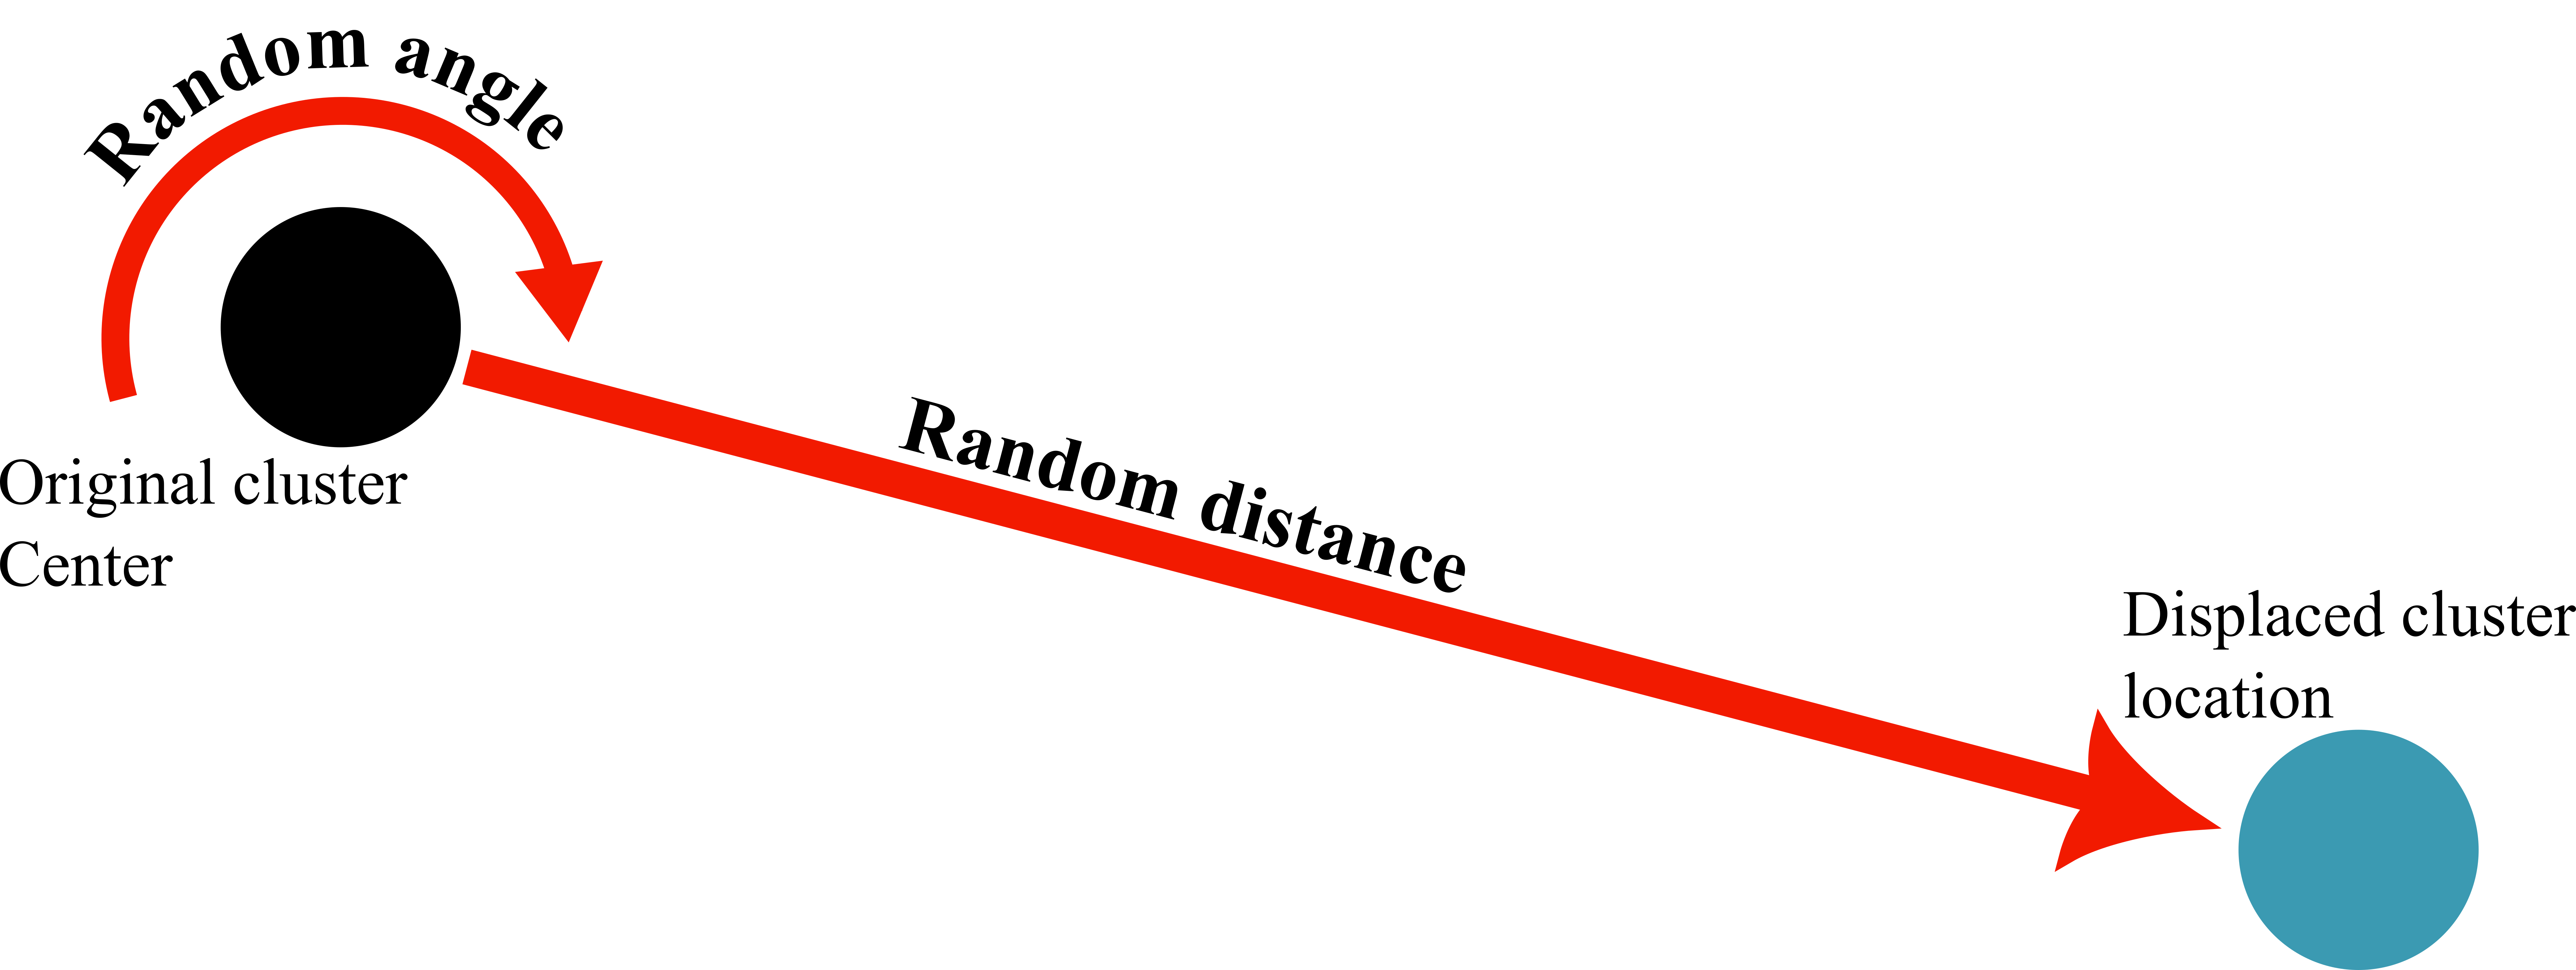
\includegraphics[width=4in]{images/displacement.png}
        \caption{DHS community / cluster displacement procedure \cite{burgert_geographic_2013}}
        \label{fig:displaceProc}
    \end{figure}    

The displacement procedure can be used to define a probability density function (PDF). Equation \ref{eq:pdf} expresses the PDF where $r$ is the limit of the radius of displacement (e.g. 2km for urban communities), and $(x_{0},y_{0})$ are the latitude and longitude distance from the 'true' community location.

\subsection{Probability density function}

    \begin{equation}
    \label{eq:pdf}
f(x_{0},y_{0}) = 
\begin{dcases}
\frac{1}{2\pi r\sqrt{x_{0}^{2}+y_{0}^{2}}}, & \text{if } \sqrt{x_{0}^2 + y_{0}^2} \leq r \\
0, & \text{otherwise}
\end{dcases}
\end{equation}

Alternatively, the symmetry of the PDF can be visualized in Figure \ref{fig:pdf_surface}. An integral of the surface shown in Figure \ref{fig:pdf_surface} gives the probability that the displaced point will fall in a defined area given the true location. Because the PDF is symmetric, integrals of the same PDF can be can be used to calculate the probability of the true location falling in a defined area given the displaced location.

    \begin{figure}[htbp]
        \centering
        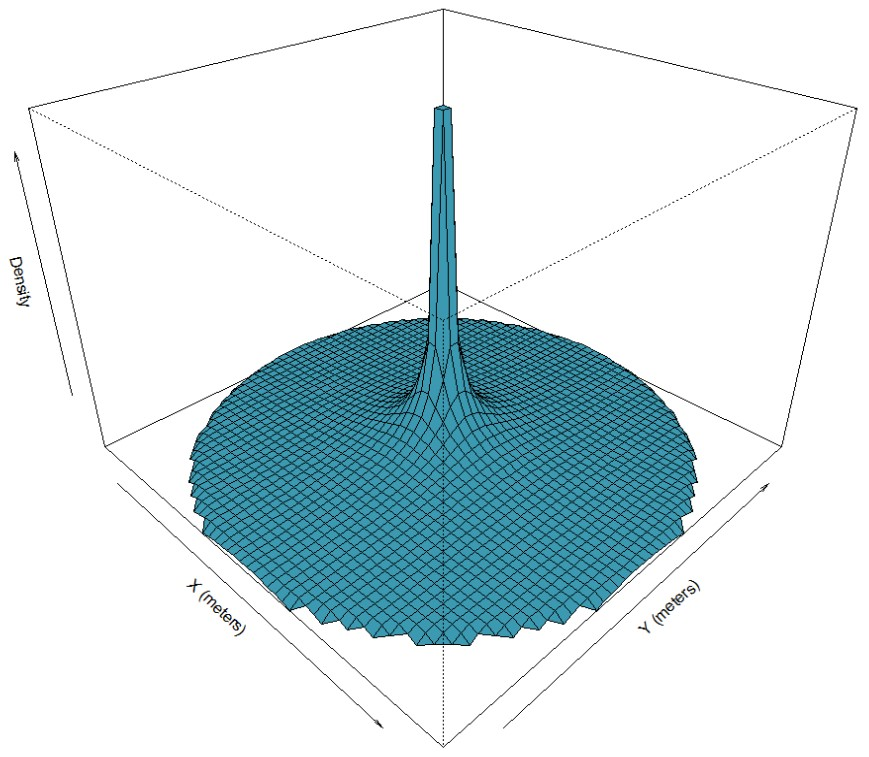
\includegraphics[width=4in]{images/DensityPlot.jpg}
        \caption{Visualization of the surface created by equation \ref{eq:pdf}, with displacement up to $r$ kilometers}
        \label{fig:pdf_surface}
    \end{figure}

Impossible locations (such as those falling outside an administrative boundary) can be trimmed from the probability buffer and the buffer re-weighted so that the volume under the surface sums to one. This buffer can be calculated for a raster at a given resolution, where the layer values are the calculated probabilities that the true cluster center falls within that cell.

To join using the probabilistic approach, a probability raster can be calculated for each displaced community location. A join can be made at the center point of each cell $(x,y)$, and the result of each join at cell $(x,y)$ can be weighted by the probability that the true community location is contained in that cell. An analyst may take a \textbf{}{probability-weighted average} for joining displaced communities to a raster with continuous values. If joining communities to a polygon (such as the catchment area of a health facility), an analyst could use this method to select the \textbf{maximum likely polygon} that a community falls in.

\section{Simulation Study}

I evaluate the performance of the join to a raster created in AccessMod 5.0 \autocite{who_accessmod_2021}, where cell values were travel time in minutes to the nearest health facility from the 2018 SPA. The simulation procedure follows these steps:

Performance is assessed by 1) setting a "true" location and value, 2) applying the DHS displacement algorithm on the true location, 3) applying established linking methods and the proposed probability-based method, and 4) comparing the error and bias of the established method with the probability-based method \autocite{morris_using_2019}.

\begin{enumerate}
    \item Set a "true" location, and value / join at that location. In this case, I treat the given locations of community locations from the 2016-2017 Haiti DHS as true.
    \item Next, I apply the DHS displacement algorithm on the true location - each time a displacement is performed is referred to as an iteration. I perform 50 Monte Carlo simulations of displacement for 298 DHS community locations based on the procedure outlined in Figure \ref{fig:displaceProc} for 14900 total simulations.
    \item I link each iteration to the spatial raster surface using the mainstream, or conventional methods \textit{and} the using proposed probability-based method.
    \item I compare performance of the established method with the probability-based method based on the error and bias \autocite{morris_using_2019}.
\end{enumerate}

% \section{Case Study (?)}

% I fit multilevel logistic regression models to predict 4+ antenatal care visits and current use of a modern family planning (MFP) method using probability-weighted median (PWM) of travel time to health facility. Service Readiness Index (SRI) Scores approaches can be compared, where Buffer Mean (BM) used the conventional simple average of health facility scores within 10km, and PWM was the mean score weighted by the probability that the true location was in a health facility's catchment area. Models adjusted for demographic characteristics and included community-specific random effects. 

% I test the performance of the simulation with other raster surfaces, either randomly generated (varying the level of spatial autocorrelation), or using measurements like temperature, precipitation, etc.

\chapter{Health Service Environment \& Service Utilization}
\label{ch:hseUtilization}

\section{Data}

This analysis will be most feasible in countries where there is a census of health facilities included in the SPA. These include Malawi and Haiti. Haiti may be preferable, as the SPA and DHS were conducted twice there (2014 and 2017), allowing for additional, confirmatory analysis.

\subsection{Service Provision Assessment}

In eligible countries, the Service Provision Assessment is a census of health facilities. It includes detailed information about health facilities, their staff, medical stock, services offered, and infrastructure.

\subsection{Demographic and Health Survey}

The Demographic and Health Surveys are household surveys that collect information about household characteristics, health attitudes, behaviors and outcomes, and more. Households are selected using a two-stage stratified sampling approach. First, sample sizes within each strata are set such that they provide commonly used indicators sufficient precision. Next, communities (or census blocks, which I will refer to as communities) are selected with probability proportional to size. Households are the ultimate sampling unit, and are selected using systematic random sampling from a count of all households in selected communities.

Every eligible respondent (typically men and women of reproductive age) who slept in the household the night before the survey visit is interviewed.

GPS points are taken for at the center of the community, and displaced according to the procedure described in Section \ref{sec:dispProc}.

\section{Linking SPA to the DHS}
\label{sec:linking}

First I will define a catchment area for health facilities. This may be accomplished by using Thiessen polygons (Thiessen polygons define the area where a health facility would be the closest by euclidean distance) or an access score using an enhanced two step floating catchment area \autocite{gao_understanding_2019-1}, or the traditional method of simply drawing a buffer around a health facility.

Next, using the distribution described in Equation \ref{eq:pdf} and Figure \ref{fig:pdf_surface}, I will calculate the average access or quality score of health facilities weighted by the probability that a community falls within that facility's catchment area (in the case of a the Thiessen polygon approach), or the probability of an access score (in the case of the two-step floating catchment area approach).

\section{Analytic approach}

\subsection{Dependent variables}

\begin{itemize}
    \item Antenatal care for most recent pregnancy
    \begin{itemize}
        \item Full antenatal care: defined as attending four or more ANC visits
        \item Timely initiation of Antenatal Care: Defined as first visit within the first trimester
    \end{itemize}
    \item Facility-based delivery among births in the past five years
    \item Care-seeking for children younger than five years with fever or diarrhea.
    \item Use of informal providers
\end{itemize}

\subsection{Independent Variables}

\begin{itemize}
    \item Access score (derived with the linking approach described in Section \ref{sec:linking})
    \begin{itemize}
        \item Weighted quality approach
        \item Weighted E2SFCA access score (with SRI measure of quality as capacity, similar to \cite{gao_understanding_2019})
    \end{itemize}
    \item Individual and community characteristic
    \begin{itemize}
        \item Household wealth
        \item Education level
        \item Marital status
        \item Child / birth indicators
        \begin{itemize}
            \item (For Antenatal care outcome) Parity, age of mother at time of birth
            \item (For Sick child outcome) Age, sex of child
        \end{itemize}
    \end{itemize}
\end{itemize}


\section{Models}

I anticipate implementing a multilevel model because the households clustered within communities likely violate the assumption of independence between observations. The first level of the model will be the individual, I will set a community-specific random intercept to account for intra-community homogeneity. 


%%% conclusions %%%%%%%%%%%%%%%%%%%%%%%%%%%%%%%%%%%%%%%%%%%%%%%%%%%%%%%%
\chapter{Conclusions}
  \label{ch:conclusions}

\graphicspath{}
\input{conclusions}

%%% bibliography %%%%%%%%%%%%%%%%%%%%%%%%%%%%%%%%%%%%%%%%%%%%%%%%%%%%%%%
%
%  \printbibliography in biblatex is great, but doesn't allow for the
%  greatest customization, so we'll use the package biblatex + biber
%  backend to meet some requirements:
%
%  * bibliography should be an un-numbered chapter, and still have a
%    pdfbookmark and a line in the table of contents
%
%  * bibliography contents should be singlespace, and optionally a smaller
%    font
%
%  * first line of this "chapter" should be in the same spot as the first
%    line of preface sections (e.g., acknowledgement)
%
%  * we use \raggedright so things like URLs and DOIs aren't stretched out.
%
\clearpage
% \chapter*{Bibliography}
% \addcontentsline{toc}{chapter}{Bibliography}
% \printbibliography{}

\begin{singlespace}
  % increase penalty such that we don't break entries over pages
  % source: https://tex.stackexchange.com/a/43275
  \patchcmd{\bibsetup}{\interlinepenalty=5000}{\interlinepenalty=10000}{}{}

  % reduce spacing between each bibentry
  \setlength\bibitemsep{0.9\baselineskip}

  % don't justify-align entries: this prevents stretching out each line
  \raggedright
  \printbibliography[
    heading = none
  ]
\end{singlespace}

\end{document}

%
% note that you'll have to modify the input file to make sure that the
% preamble (\documentclass, etc.) isn't included. to make your life
% easier, you could use some TeX conditionals to make it seamless.
%
% this requires some planning, but enables you to edit the individual
% paper and thesis chapter without tracking and porting changes between
% multiple directories and repositories:
%
% for example, at the beginning of foobar/paper.tex (before
% \documentclass):
%
%   \newif\ifdissertation
%   \dissertationtrue      % (or \dissertationfalse for the standalone)
%
%   \ifdissertation
%   \else
%   \documentclass...
%   \fi
%
%   \ifdissertation
%   \else
%   \begin{document}
%   \fi
%
%   [...paper content here...]
%
%   \ifdissertation
%   \else
%   \end{document}
%   \fi

%%% chapters: lorem ipsum %%%%%%%%%%%%%%%%%%%%%%%%%%%%%%%%%%%%%%%%%%%%%%

\chapter{Determinants of Health Facility Client Satisfation in Low- and Middle- Income Countries}
\label{ch:clientSat}

\section{Introduction}

Primary health coverage is essential to building and maintaining progress on morbidity and mortality reductions, particularly in Low-and Middle-Income Countries (LMICs) where preventable deaths still rank among the most common <CITE>. A robust body of evidence has identified health service quality as a core ingredient for achieving better health outcomes \autocite{world_health_organization_delivering_2018}, but treatment success is conditional on service utilization - a construct that is largely determined by accessibility and perceptions of quality <CITE>.

\subsection{WHY IT MATTERS} %

In higher income countries, previous research has shown a relationship between client satisfaction and health service utilization \autocite{zastowny_patient_1989} <CITE MORE>. More satisfied individuals are more likely to seek care from providers. A more thorough avenue of determinants of health service utilization may offer a path to higher health service utilization.

\subsubsection{PATIENT SATISFACTION GENERALLY}

\subsubsection{PATIENT SATISFACTION IN LMICs}




\section{Methods}

\subsection{Data}

Data will be SPA data from DHS Phase VII with client exit interviews. Afghanistan, Haiti, Nepal and Tanzania meet this eligibility criteria and were the surveys were conducted between 2015 and 2018.

\subsection{Outcomes}

There are several measures of client (alternatively referred to as "patient") satisfaction available in the Service provision assessment. Each of these indicators are separately available for the three health services (antentatal care, sick child care, and family planning). For this analysis, I extract two composite indicators as key outcomes. I construct composite indicators, because in these settings, few clients report complaints or express dissatisfaction. Composite indicators enable exploration facilitate a measure of \textit{any} dissatisfaction.

\subsubsection{Client satisfaction} Two questions are used to construct this indicator. First, for each service type, the questionnaire asks "how satisfied are you with the services you recieved today." Possible responses include "very satisfied", "more or less satisfied" or "not satisfied". Second, respondents are asked whether they would recommend the facility to a friend or family member (possible responses are "yes" or "no"). If a client does not respond that they are "very satisfied" or that they would not recommend the facility to a friend, client satisfaction is coded 0, otherwise it is coded 1.

\subsubsection{Free of problems}: Clients are asked about 11 specific potential problems during their visit and whether each was a "major", "minor", or "no problem" during their visit. Items such as wait time, cost, privacy, respect, etc. The few peer reviewed studies that have examined this based on SPA data have collapsed this into a dichotomous free of problems (=1) vs. any problem (=0) problems \autocite{do_quality_2017, bergh_identifying_2022}. One relevant dissertation coded this as an additive index with values possible values between 0 and 11 \autocite{riese_associations_2019}.
    
\end{itemize}

\subsection{Independent Variables}

Several variables measuring facility level, provider level, and client demographic level, and characteristics of the provider's interaction with the client are explored as potential predictors of facility satisfaction.

\subsubsection{Service Readiness Index}

Using a dimensional reduction technique such as Principal Components Analysis (PCA), Multiple Correspondence Analysis, or Latent Class Analysis could be helpful for creating a more useful index following an approach similar to DHS wealth index calculation \autocite{dhs_program_dhs_nodate}. However, the fact that a substantial proportion of clients report satisfaction on all measures may constrain the possible analytic approaches.

\subsubsection{Provider characteristics}

\subsubsection{Client demographic characteristics}

\subsubsection{Visit observation}

\subsection{Analytic Approach}

I will likely explore a variable selection technique (such as stepwise regression) to explore determinants that are meaningfully associated with measures of satisfaction in selected countries. The initial list of included predictors will be from the service readiness index \autocite{world_health_organization_service_2014}. Regression analysis will be performed using a Bayesian framework, and I will explore the utility of each outcome.

\chapter{Linking Geomasked Demographic and Health Service Data and Other Spatial Layers: A Simulation Study}
\label{ch:simStudy}

\section{Data}

This study can be conducted in countries that have a census of health facilities included in the Service Provision Assessment and a corresponding Demographic \& Health Survey. Malawi and Haiti meet this criteria. The first version of the paper was based on Haiti.

\section{DHS geomasking}

\subsection{Displacement Procedure}
\label{subsubsec:dispProc}

The displacement procedure is shown in Figure \ref{fig:displaceProc}. First a random angle is selected, then a random distance up to a limit depending on the community type. Urban communities are displaced up to 2km, rural are displaced up to 5km with a 1\% chance of being displaced up to 10km. If a community is displaced point outside of its original administrative boundary, then the displacement procedure is \textbf{repeated} for that community.

    \begin{figure}[htbp]
        \centering
        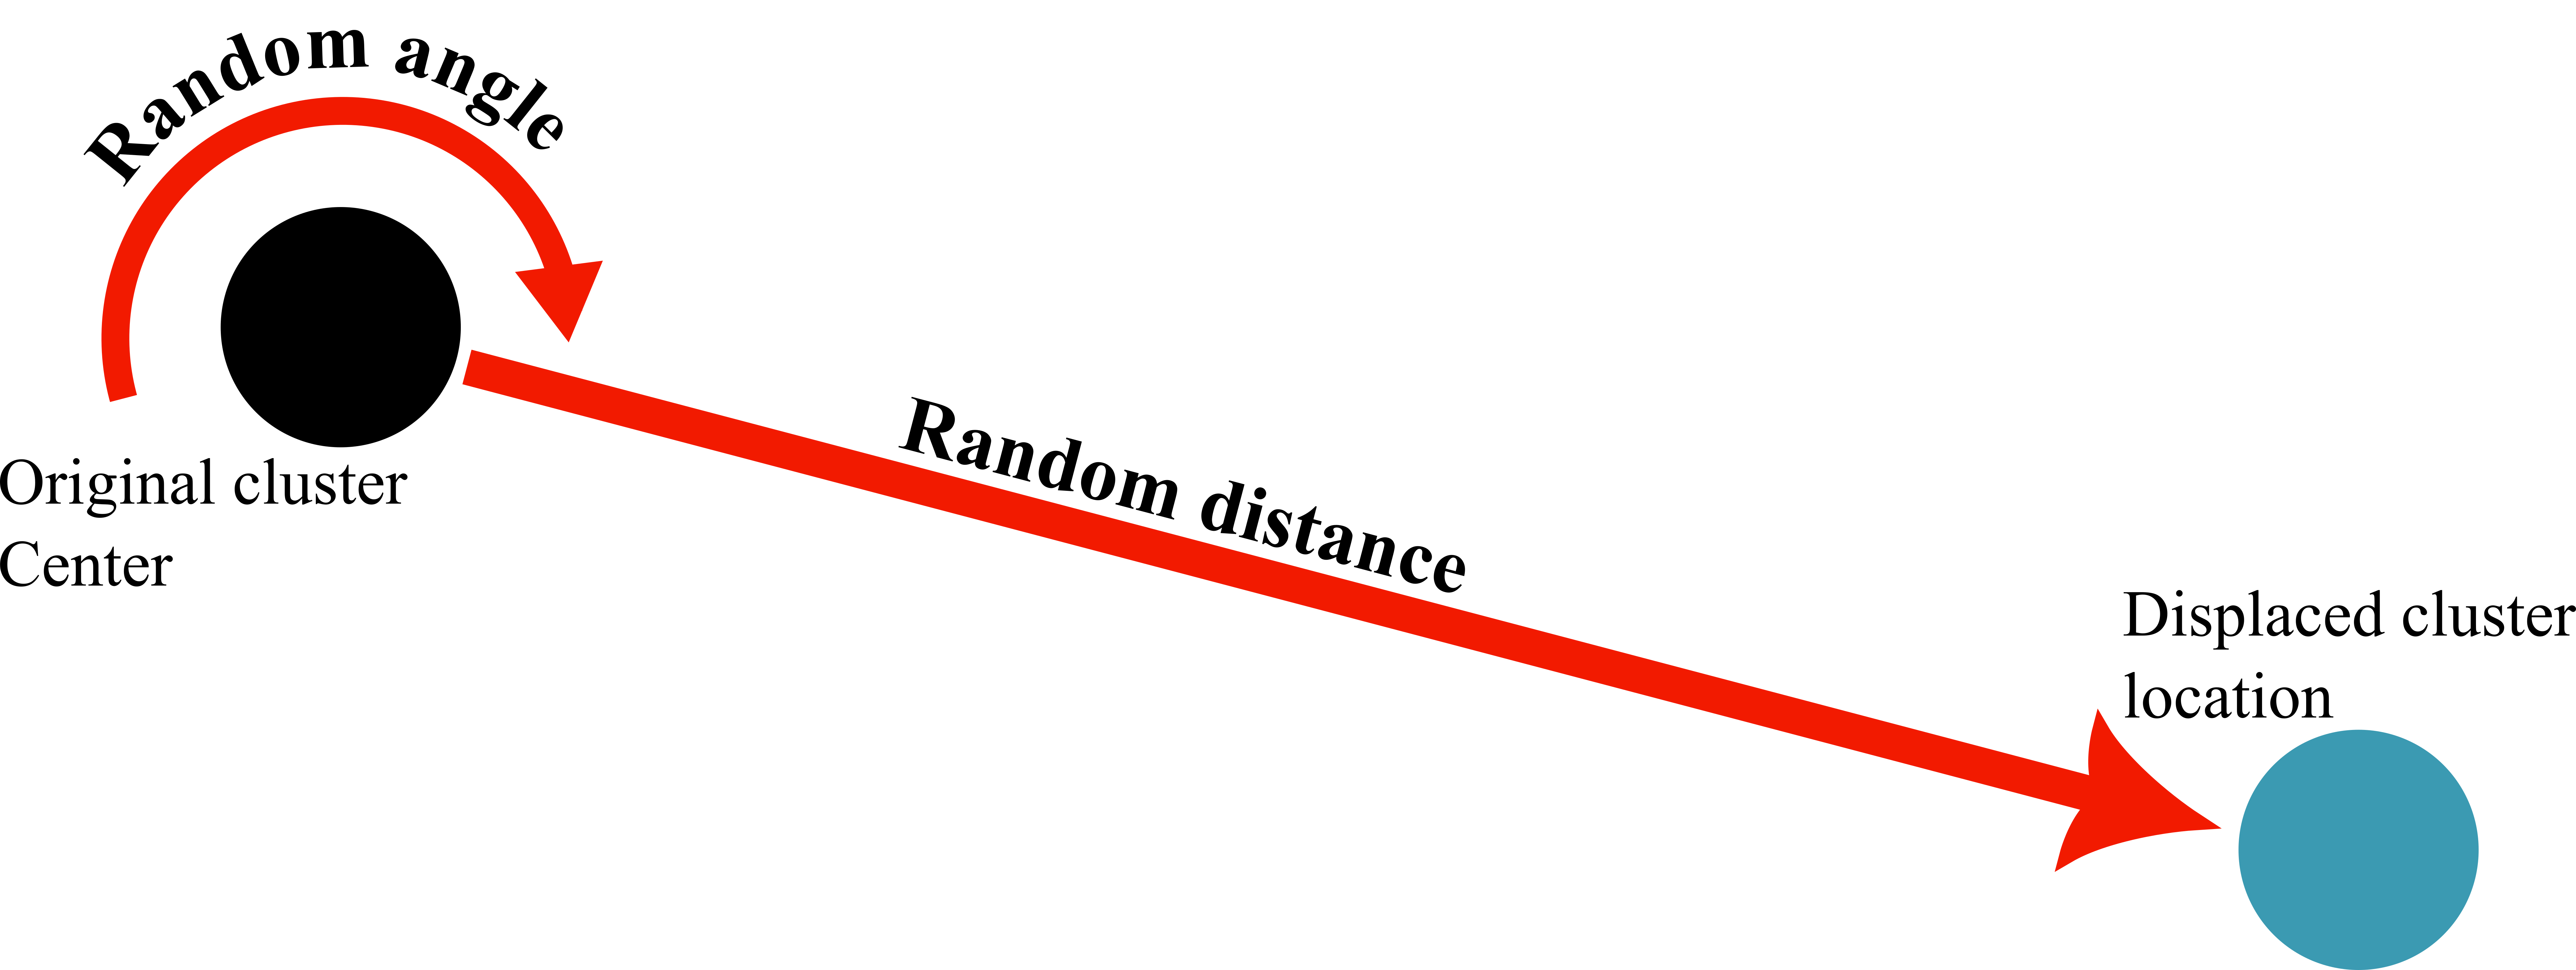
\includegraphics[width=4in]{images/displacement.png}
        \caption{DHS community / cluster displacement procedure \cite{burgert_geographic_2013}}
        \label{fig:displaceProc}
    \end{figure}    

The displacement procedure can be used to define a probability density function (PDF). Equation \ref{eq:pdf} expresses the PDF where $r$ is the limit of the radius of displacement (e.g. 2km for urban communities), and $(x_{0},y_{0})$ are the latitude and longitude distance from the 'true' community location.

\subsection{Probability density function}

    \begin{equation}
    \label{eq:pdf}
f(x_{0},y_{0}) = 
\begin{dcases}
\frac{1}{2\pi r\sqrt{x_{0}^{2}+y_{0}^{2}}}, & \text{if } \sqrt{x_{0}^2 + y_{0}^2} \leq r \\
0, & \text{otherwise}
\end{dcases}
\end{equation}

Alternatively, the symmetry of the PDF can be visualized in Figure \ref{fig:pdf_surface}. An integral of the surface shown in Figure \ref{fig:pdf_surface} gives the probability that the displaced point will fall in a defined area given the true location. Because the PDF is symmetric, integrals of the same PDF can be can be used to calculate the probability of the true location falling in a defined area given the displaced location.

    \begin{figure}[htbp]
        \centering
        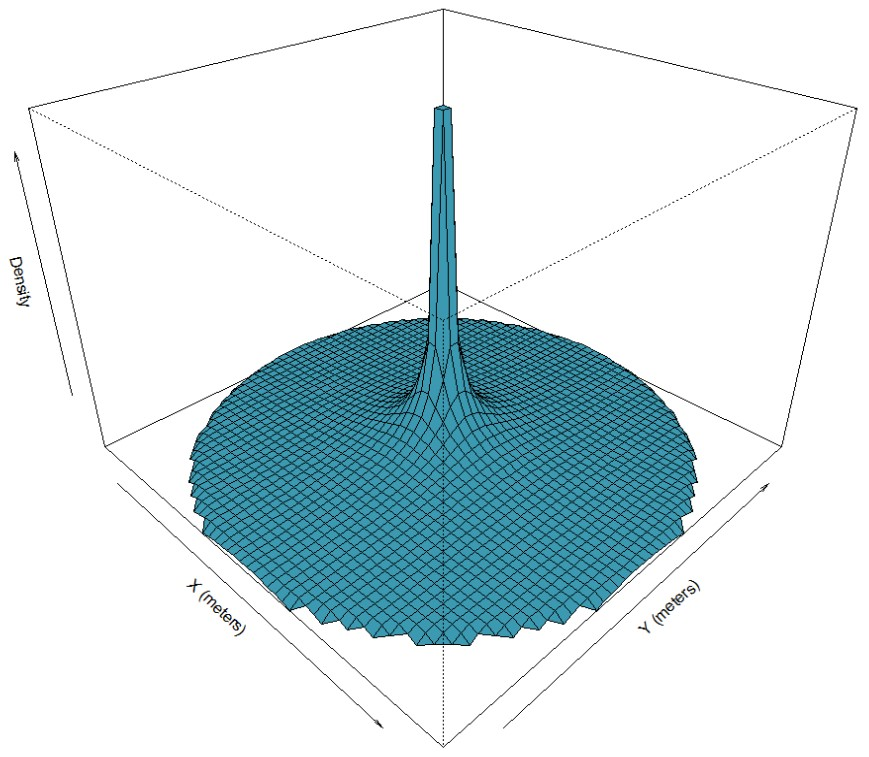
\includegraphics[width=4in]{images/DensityPlot.jpg}
        \caption{Visualization of the surface created by equation \ref{eq:pdf}, with displacement up to $r$ kilometers}
        \label{fig:pdf_surface}
    \end{figure}

Impossible locations (such as those falling outside an administrative boundary) can be trimmed from the probability buffer and the buffer re-weighted so that the volume under the surface sums to one. This buffer can be calculated for a raster at a given resolution, where the layer values are the calculated probabilities that the true cluster center falls within that cell.

To join using the probabilistic approach, a probability raster can be calculated for each displaced community location. A join can be made at the center point of each cell $(x,y)$, and the result of each join at cell $(x,y)$ can be weighted by the probability that the true community location is contained in that cell. An analyst may take a \textbf{}{probability-weighted average} for joining displaced communities to a raster with continuous values. If joining communities to a polygon (such as the catchment area of a health facility), an analyst could use this method to select the \textbf{maximum likely polygon} that a community falls in.

\section{Simulation Study}

I evaluate the performance of the join to a raster created in AccessMod 5.0 \autocite{who_accessmod_2021}, where cell values were travel time in minutes to the nearest health facility from the 2018 SPA. The simulation procedure follows these steps:

Performance is assessed by 1) setting a "true" location and value, 2) applying the DHS displacement algorithm on the true location, 3) applying established linking methods and the proposed probability-based method, and 4) comparing the error and bias of the established method with the probability-based method \autocite{morris_using_2019}.

\begin{enumerate}
    \item Set a "true" location, and value / join at that location. In this case, I treat the given locations of community locations from the 2016-2017 Haiti DHS as true.
    \item Next, I apply the DHS displacement algorithm on the true location - each time a displacement is performed is referred to as an iteration. I perform 50 Monte Carlo simulations of displacement for 298 DHS community locations based on the procedure outlined in Figure \ref{fig:displaceProc} for 14900 total simulations.
    \item I link each iteration to the spatial raster surface using the mainstream, or conventional methods \textit{and} the using proposed probability-based method.
    \item I compare performance of the established method with the probability-based method based on the error and bias \autocite{morris_using_2019}.
\end{enumerate}

% \section{Case Study (?)}

% I fit multilevel logistic regression models to predict 4+ antenatal care visits and current use of a modern family planning (MFP) method using probability-weighted median (PWM) of travel time to health facility. Service Readiness Index (SRI) Scores approaches can be compared, where Buffer Mean (BM) used the conventional simple average of health facility scores within 10km, and PWM was the mean score weighted by the probability that the true location was in a health facility's catchment area. Models adjusted for demographic characteristics and included community-specific random effects. 

% I test the performance of the simulation with other raster surfaces, either randomly generated (varying the level of spatial autocorrelation), or using measurements like temperature, precipitation, etc.

\chapter{Health Service Environment \& Service Utilization}
\label{ch:hseUtilization}

\section{Data}

This analysis will be most feasible in countries where there is a census of health facilities included in the SPA. These include Malawi and Haiti. Haiti may be preferable, as the SPA and DHS were conducted twice there (2014 and 2017), allowing for additional, confirmatory analysis.

\subsection{Service Provision Assessment}

In eligible countries, the Service Provision Assessment is a census of health facilities. It includes detailed information about health facilities, their staff, medical stock, services offered, and infrastructure.

\subsection{Demographic and Health Survey}

The Demographic and Health Surveys are household surveys that collect information about household characteristics, health attitudes, behaviors and outcomes, and more. Households are selected using a two-stage stratified sampling approach. First, sample sizes within each strata are set such that they provide commonly used indicators sufficient precision. Next, communities (or census blocks, which I will refer to as communities) are selected with probability proportional to size. Households are the ultimate sampling unit, and are selected using systematic random sampling from a count of all households in selected communities.

Every eligible respondent (typically men and women of reproductive age) who slept in the household the night before the survey visit is interviewed.

GPS points are taken for at the center of the community, and displaced according to the procedure described in Section \ref{sec:dispProc}.

\section{Linking SPA to the DHS}
\label{sec:linking}

First I will define a catchment area for health facilities. This may be accomplished by using Thiessen polygons (Thiessen polygons define the area where a health facility would be the closest by euclidean distance) or an access score using an enhanced two step floating catchment area \autocite{gao_understanding_2019-1}, or the traditional method of simply drawing a buffer around a health facility.

Next, using the distribution described in Equation \ref{eq:pdf} and Figure \ref{fig:pdf_surface}, I will calculate the average access or quality score of health facilities weighted by the probability that a community falls within that facility's catchment area (in the case of a the Thiessen polygon approach), or the probability of an access score (in the case of the two-step floating catchment area approach).

\section{Analytic approach}

\subsection{Dependent variables}

\begin{itemize}
    \item Antenatal care for most recent pregnancy
    \begin{itemize}
        \item Full antenatal care: defined as attending four or more ANC visits
        \item Timely initiation of Antenatal Care: Defined as first visit within the first trimester
    \end{itemize}
    \item Facility-based delivery among births in the past five years
    \item Care-seeking for children younger than five years with fever or diarrhea.
    \item Use of informal providers
\end{itemize}

\subsection{Independent Variables}

\begin{itemize}
    \item Access score (derived with the linking approach described in Section \ref{sec:linking})
    \begin{itemize}
        \item Weighted quality approach
        \item Weighted E2SFCA access score (with SRI measure of quality as capacity, similar to \cite{gao_understanding_2019})
    \end{itemize}
    \item Individual and community characteristic
    \begin{itemize}
        \item Household wealth
        \item Education level
        \item Marital status
        \item Child / birth indicators
        \begin{itemize}
            \item (For Antenatal care outcome) Parity, age of mother at time of birth
            \item (For Sick child outcome) Age, sex of child
        \end{itemize}
    \end{itemize}
\end{itemize}


\section{Models}

I anticipate implementing a multilevel model because the households clustered within communities likely violate the assumption of independence between observations. The first level of the model will be the individual, I will set a community-specific random intercept to account for intra-community homogeneity. 


%%% conclusions %%%%%%%%%%%%%%%%%%%%%%%%%%%%%%%%%%%%%%%%%%%%%%%%%%%%%%%%
\chapter{Conclusions}
  \label{ch:conclusions}

\graphicspath{}
\input{conclusions}

%%% bibliography %%%%%%%%%%%%%%%%%%%%%%%%%%%%%%%%%%%%%%%%%%%%%%%%%%%%%%%
%
%  \printbibliography in biblatex is great, but doesn't allow for the
%  greatest customization, so we'll use the package biblatex + biber
%  backend to meet some requirements:
%
%  * bibliography should be an un-numbered chapter, and still have a
%    pdfbookmark and a line in the table of contents
%
%  * bibliography contents should be singlespace, and optionally a smaller
%    font
%
%  * first line of this "chapter" should be in the same spot as the first
%    line of preface sections (e.g., acknowledgement)
%
%  * we use \raggedright so things like URLs and DOIs aren't stretched out.
%
\clearpage
% \chapter*{Bibliography}
% \addcontentsline{toc}{chapter}{Bibliography}
% \printbibliography{}

\begin{singlespace}
  % increase penalty such that we don't break entries over pages
  % source: https://tex.stackexchange.com/a/43275
  \patchcmd{\bibsetup}{\interlinepenalty=5000}{\interlinepenalty=10000}{}{}

  % reduce spacing between each bibentry
  \setlength\bibitemsep{0.9\baselineskip}

  % don't justify-align entries: this prevents stretching out each line
  \raggedright
  \printbibliography[
    heading = none
  ]
\end{singlespace}

\end{document}

%
% note that you'll have to modify the input file to make sure that the
% preamble (\documentclass, etc.) isn't included. to make your life
% easier, you could use some TeX conditionals to make it seamless.
%
% this requires some planning, but enables you to edit the individual
% paper and thesis chapter without tracking and porting changes between
% multiple directories and repositories:
%
% for example, at the beginning of foobar/paper.tex (before
% \documentclass):
%
%   \newif\ifdissertation
%   \dissertationtrue      % (or \dissertationfalse for the standalone)
%
%   \ifdissertation
%   \else
%   \documentclass...
%   \fi
%
%   \ifdissertation
%   \else
%   \begin{document}
%   \fi
%
%   [...paper content here...]
%
%   \ifdissertation
%   \else
%   \end{document}
%   \fi

%%% chapters: lorem ipsum %%%%%%%%%%%%%%%%%%%%%%%%%%%%%%%%%%%%%%%%%%%%%%

\chapter{Determinants of Health Facility Client Satisfation in Low- and Middle- Income Countries}
\label{ch:clientSat}

\section{Introduction}

Primary health coverage is essential to building and maintaining progress on morbidity and mortality reductions, particularly in Low-and Middle-Income Countries (LMICs) where preventable deaths still rank among the most common <CITE>. A robust body of evidence has identified health service quality as a core ingredient for achieving better health outcomes \autocite{world_health_organization_delivering_2018}, but treatment success is conditional on service utilization - a construct that is largely determined by accessibility and perceptions of quality <CITE>.

\subsection{WHY IT MATTERS} %

In higher income countries, previous research has shown a relationship between client satisfaction and health service utilization \autocite{zastowny_patient_1989} <CITE MORE>. More satisfied individuals are more likely to seek care from providers. A more thorough avenue of determinants of health service utilization may offer a path to higher health service utilization.

\subsubsection{PATIENT SATISFACTION GENERALLY}

\subsubsection{PATIENT SATISFACTION IN LMICs}




\section{Methods}

\subsection{Data}

Data will be SPA data from DHS Phase VII with client exit interviews. Afghanistan, Haiti, Nepal and Tanzania meet this eligibility criteria and were the surveys were conducted between 2015 and 2018.

\subsection{Outcomes}

There are several measures of client (alternatively referred to as "patient") satisfaction available in the Service provision assessment. Each of these indicators are separately available for the three health services (antentatal care, sick child care, and family planning). For this analysis, I extract two composite indicators as key outcomes. I construct composite indicators, because in these settings, few clients report complaints or express dissatisfaction. Composite indicators enable exploration facilitate a measure of \textit{any} dissatisfaction.

\subsubsection{Client satisfaction} Two questions are used to construct this indicator. First, for each service type, the questionnaire asks "how satisfied are you with the services you recieved today." Possible responses include "very satisfied", "more or less satisfied" or "not satisfied". Second, respondents are asked whether they would recommend the facility to a friend or family member (possible responses are "yes" or "no"). If a client does not respond that they are "very satisfied" or that they would not recommend the facility to a friend, client satisfaction is coded 0, otherwise it is coded 1.

\subsubsection{Free of problems}: Clients are asked about 11 specific potential problems during their visit and whether each was a "major", "minor", or "no problem" during their visit. Items such as wait time, cost, privacy, respect, etc. The few peer reviewed studies that have examined this based on SPA data have collapsed this into a dichotomous free of problems (=1) vs. any problem (=0) problems \autocite{do_quality_2017, bergh_identifying_2022}. One relevant dissertation coded this as an additive index with values possible values between 0 and 11 \autocite{riese_associations_2019}.
    
\end{itemize}

\subsection{Independent Variables}

Several variables measuring facility level, provider level, and client demographic level, and characteristics of the provider's interaction with the client are explored as potential predictors of facility satisfaction.

\subsubsection{Service Readiness Index}

Using a dimensional reduction technique such as Principal Components Analysis (PCA), Multiple Correspondence Analysis, or Latent Class Analysis could be helpful for creating a more useful index following an approach similar to DHS wealth index calculation \autocite{dhs_program_dhs_nodate}. However, the fact that a substantial proportion of clients report satisfaction on all measures may constrain the possible analytic approaches.

\subsubsection{Provider characteristics}

\subsubsection{Client demographic characteristics}

\subsubsection{Visit observation}

\subsection{Analytic Approach}

I will likely explore a variable selection technique (such as stepwise regression) to explore determinants that are meaningfully associated with measures of satisfaction in selected countries. The initial list of included predictors will be from the service readiness index \autocite{world_health_organization_service_2014}. Regression analysis will be performed using a Bayesian framework, and I will explore the utility of each outcome.

\chapter{Linking Geomasked Demographic and Health Service Data and Other Spatial Layers: A Simulation Study}
\label{ch:simStudy}

\section{Data}

This study can be conducted in countries that have a census of health facilities included in the Service Provision Assessment and a corresponding Demographic \& Health Survey. Malawi and Haiti meet this criteria. The first version of the paper was based on Haiti.

\section{DHS geomasking}

\subsection{Displacement Procedure}
\label{subsubsec:dispProc}

The displacement procedure is shown in Figure \ref{fig:displaceProc}. First a random angle is selected, then a random distance up to a limit depending on the community type. Urban communities are displaced up to 2km, rural are displaced up to 5km with a 1\% chance of being displaced up to 10km. If a community is displaced point outside of its original administrative boundary, then the displacement procedure is \textbf{repeated} for that community.

    \begin{figure}[htbp]
        \centering
        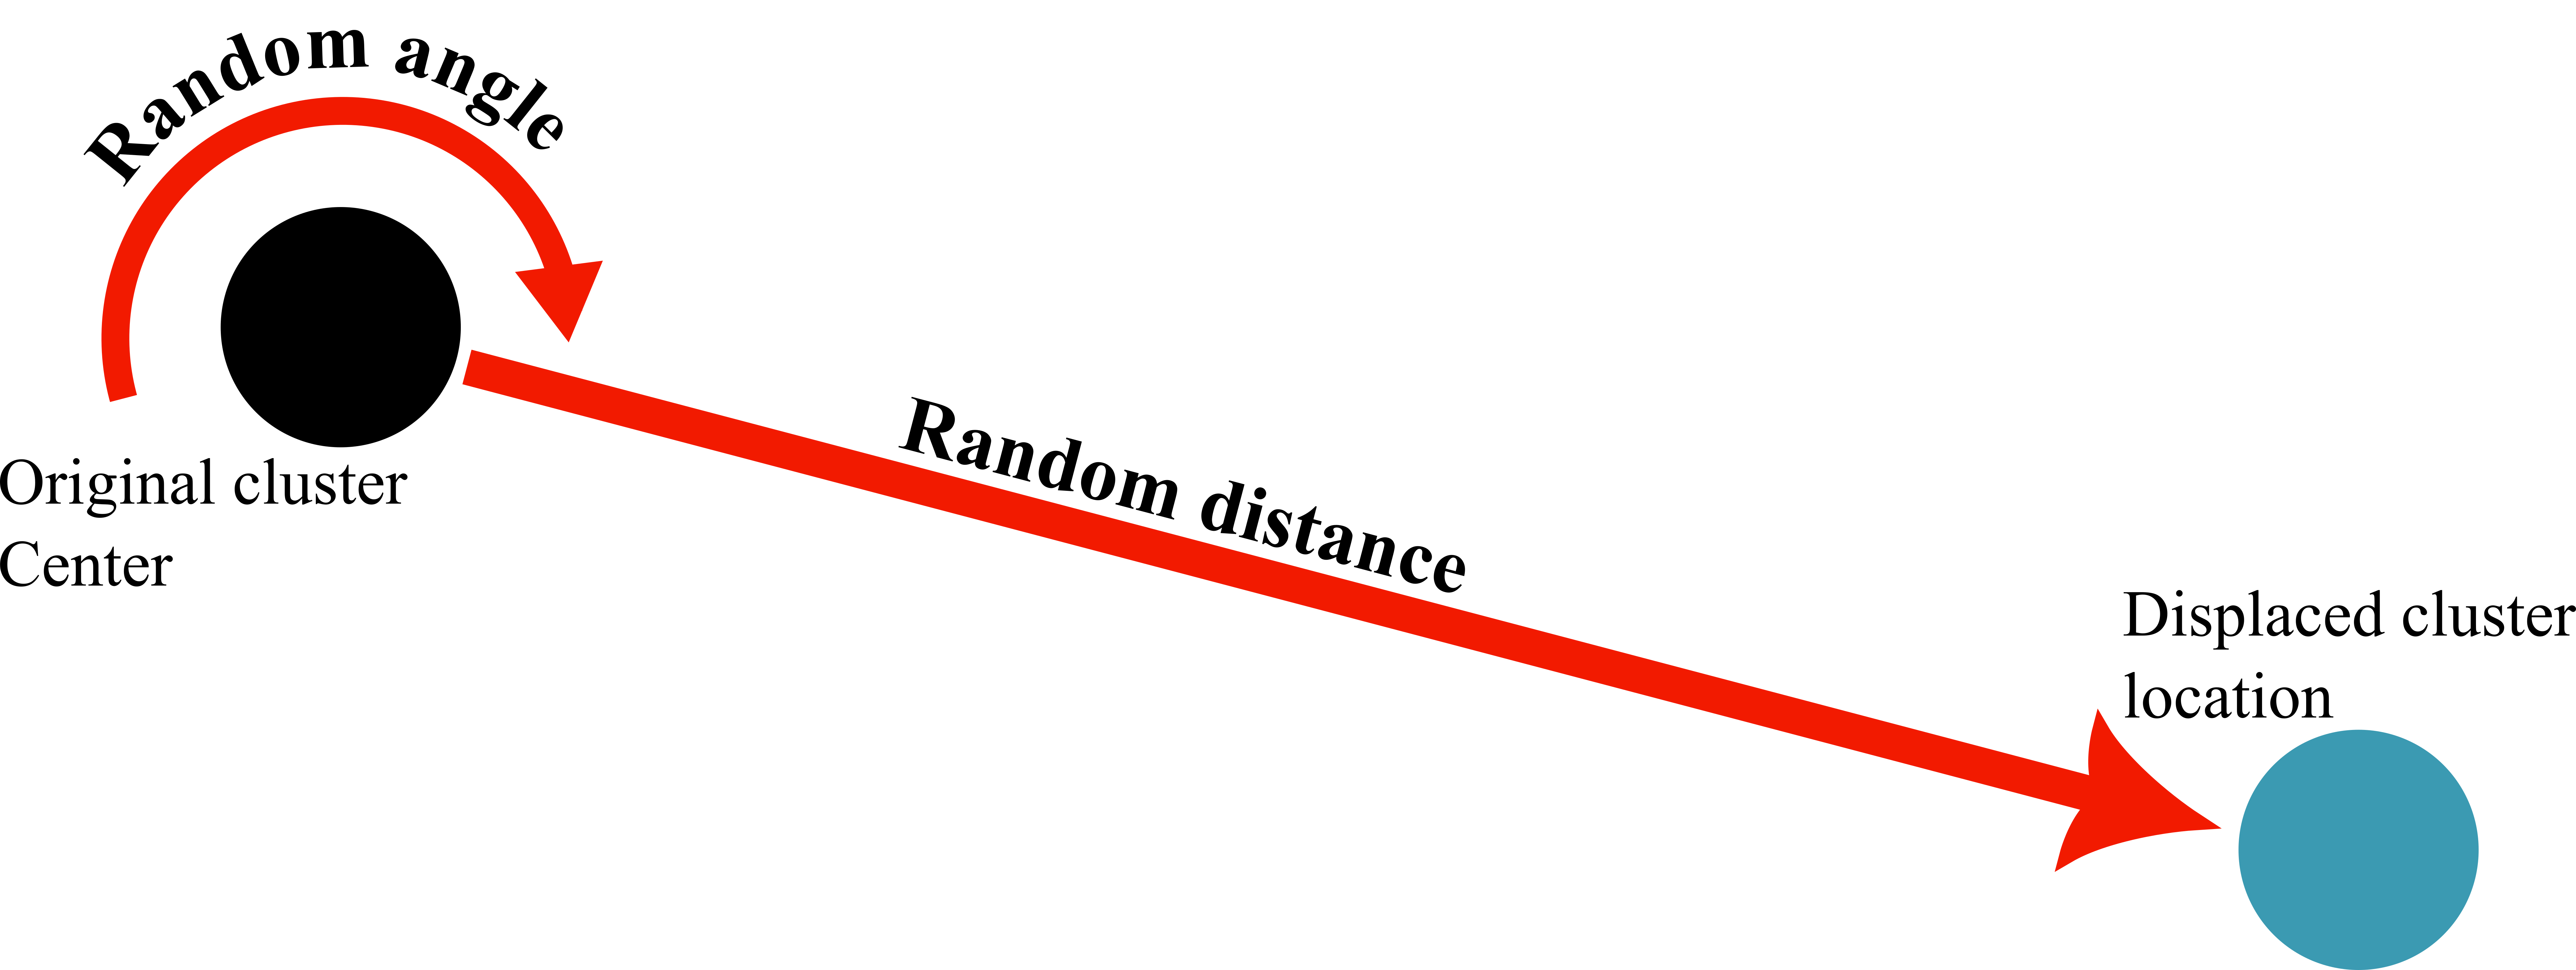
\includegraphics[width=4in]{images/displacement.png}
        \caption{DHS community / cluster displacement procedure \cite{burgert_geographic_2013}}
        \label{fig:displaceProc}
    \end{figure}    

The displacement procedure can be used to define a probability density function (PDF). Equation \ref{eq:pdf} expresses the PDF where $r$ is the limit of the radius of displacement (e.g. 2km for urban communities), and $(x_{0},y_{0})$ are the latitude and longitude distance from the 'true' community location.

\subsection{Probability density function}

    \begin{equation}
    \label{eq:pdf}
f(x_{0},y_{0}) = 
\begin{dcases}
\frac{1}{2\pi r\sqrt{x_{0}^{2}+y_{0}^{2}}}, & \text{if } \sqrt{x_{0}^2 + y_{0}^2} \leq r \\
0, & \text{otherwise}
\end{dcases}
\end{equation}

Alternatively, the symmetry of the PDF can be visualized in Figure \ref{fig:pdf_surface}. An integral of the surface shown in Figure \ref{fig:pdf_surface} gives the probability that the displaced point will fall in a defined area given the true location. Because the PDF is symmetric, integrals of the same PDF can be can be used to calculate the probability of the true location falling in a defined area given the displaced location.

    \begin{figure}[htbp]
        \centering
        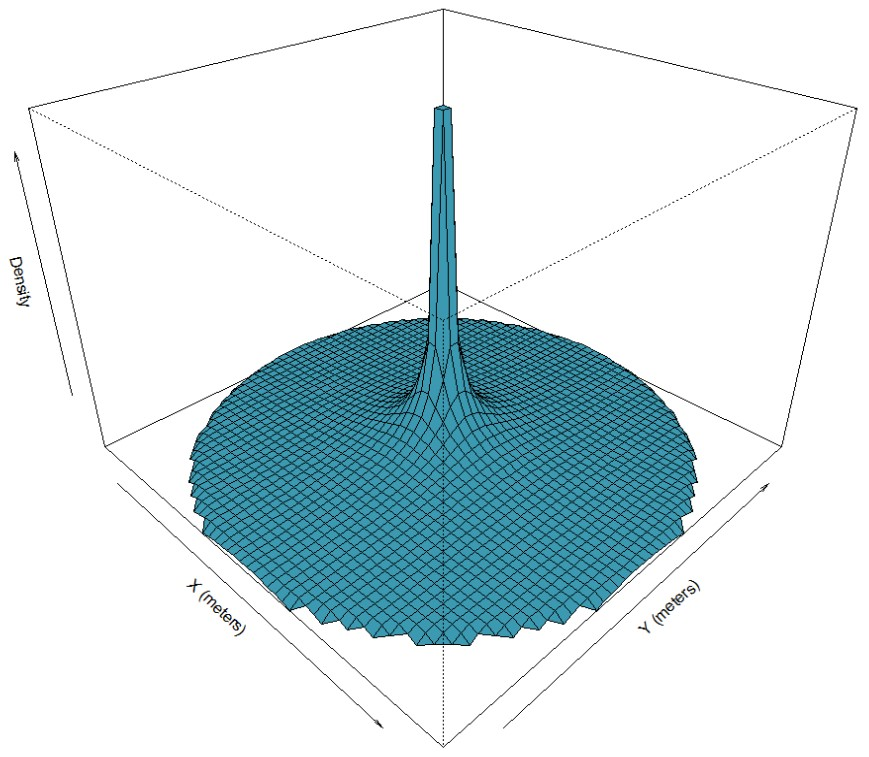
\includegraphics[width=4in]{images/DensityPlot.jpg}
        \caption{Visualization of the surface created by equation \ref{eq:pdf}, with displacement up to $r$ kilometers}
        \label{fig:pdf_surface}
    \end{figure}

Impossible locations (such as those falling outside an administrative boundary) can be trimmed from the probability buffer and the buffer re-weighted so that the volume under the surface sums to one. This buffer can be calculated for a raster at a given resolution, where the layer values are the calculated probabilities that the true cluster center falls within that cell.

To join using the probabilistic approach, a probability raster can be calculated for each displaced community location. A join can be made at the center point of each cell $(x,y)$, and the result of each join at cell $(x,y)$ can be weighted by the probability that the true community location is contained in that cell. An analyst may take a \textbf{}{probability-weighted average} for joining displaced communities to a raster with continuous values. If joining communities to a polygon (such as the catchment area of a health facility), an analyst could use this method to select the \textbf{maximum likely polygon} that a community falls in.

\section{Simulation Study}

I evaluate the performance of the join to a raster created in AccessMod 5.0 \autocite{who_accessmod_2021}, where cell values were travel time in minutes to the nearest health facility from the 2018 SPA. The simulation procedure follows these steps:

Performance is assessed by 1) setting a "true" location and value, 2) applying the DHS displacement algorithm on the true location, 3) applying established linking methods and the proposed probability-based method, and 4) comparing the error and bias of the established method with the probability-based method \autocite{morris_using_2019}.

\begin{enumerate}
    \item Set a "true" location, and value / join at that location. In this case, I treat the given locations of community locations from the 2016-2017 Haiti DHS as true.
    \item Next, I apply the DHS displacement algorithm on the true location - each time a displacement is performed is referred to as an iteration. I perform 50 Monte Carlo simulations of displacement for 298 DHS community locations based on the procedure outlined in Figure \ref{fig:displaceProc} for 14900 total simulations.
    \item I link each iteration to the spatial raster surface using the mainstream, or conventional methods \textit{and} the using proposed probability-based method.
    \item I compare performance of the established method with the probability-based method based on the error and bias \autocite{morris_using_2019}.
\end{enumerate}

% \section{Case Study (?)}

% I fit multilevel logistic regression models to predict 4+ antenatal care visits and current use of a modern family planning (MFP) method using probability-weighted median (PWM) of travel time to health facility. Service Readiness Index (SRI) Scores approaches can be compared, where Buffer Mean (BM) used the conventional simple average of health facility scores within 10km, and PWM was the mean score weighted by the probability that the true location was in a health facility's catchment area. Models adjusted for demographic characteristics and included community-specific random effects. 

% I test the performance of the simulation with other raster surfaces, either randomly generated (varying the level of spatial autocorrelation), or using measurements like temperature, precipitation, etc.

\chapter{Health Service Environment \& Service Utilization}
\label{ch:hseUtilization}

\section{Data}

This analysis will be most feasible in countries where there is a census of health facilities included in the SPA. These include Malawi and Haiti. Haiti may be preferable, as the SPA and DHS were conducted twice there (2014 and 2017), allowing for additional, confirmatory analysis.

\subsection{Service Provision Assessment}

In eligible countries, the Service Provision Assessment is a census of health facilities. It includes detailed information about health facilities, their staff, medical stock, services offered, and infrastructure.

\subsection{Demographic and Health Survey}

The Demographic and Health Surveys are household surveys that collect information about household characteristics, health attitudes, behaviors and outcomes, and more. Households are selected using a two-stage stratified sampling approach. First, sample sizes within each strata are set such that they provide commonly used indicators sufficient precision. Next, communities (or census blocks, which I will refer to as communities) are selected with probability proportional to size. Households are the ultimate sampling unit, and are selected using systematic random sampling from a count of all households in selected communities.

Every eligible respondent (typically men and women of reproductive age) who slept in the household the night before the survey visit is interviewed.

GPS points are taken for at the center of the community, and displaced according to the procedure described in Section \ref{sec:dispProc}.

\section{Linking SPA to the DHS}
\label{sec:linking}

First I will define a catchment area for health facilities. This may be accomplished by using Thiessen polygons (Thiessen polygons define the area where a health facility would be the closest by euclidean distance) or an access score using an enhanced two step floating catchment area \autocite{gao_understanding_2019-1}, or the traditional method of simply drawing a buffer around a health facility.

Next, using the distribution described in Equation \ref{eq:pdf} and Figure \ref{fig:pdf_surface}, I will calculate the average access or quality score of health facilities weighted by the probability that a community falls within that facility's catchment area (in the case of a the Thiessen polygon approach), or the probability of an access score (in the case of the two-step floating catchment area approach).

\section{Analytic approach}

\subsection{Dependent variables}

\begin{itemize}
    \item Antenatal care for most recent pregnancy
    \begin{itemize}
        \item Full antenatal care: defined as attending four or more ANC visits
        \item Timely initiation of Antenatal Care: Defined as first visit within the first trimester
    \end{itemize}
    \item Facility-based delivery among births in the past five years
    \item Care-seeking for children younger than five years with fever or diarrhea.
    \item Use of informal providers
\end{itemize}

\subsection{Independent Variables}

\begin{itemize}
    \item Access score (derived with the linking approach described in Section \ref{sec:linking})
    \begin{itemize}
        \item Weighted quality approach
        \item Weighted E2SFCA access score (with SRI measure of quality as capacity, similar to \cite{gao_understanding_2019})
    \end{itemize}
    \item Individual and community characteristic
    \begin{itemize}
        \item Household wealth
        \item Education level
        \item Marital status
        \item Child / birth indicators
        \begin{itemize}
            \item (For Antenatal care outcome) Parity, age of mother at time of birth
            \item (For Sick child outcome) Age, sex of child
        \end{itemize}
    \end{itemize}
\end{itemize}


\section{Models}

I anticipate implementing a multilevel model because the households clustered within communities likely violate the assumption of independence between observations. The first level of the model will be the individual, I will set a community-specific random intercept to account for intra-community homogeneity. 


%%% conclusions %%%%%%%%%%%%%%%%%%%%%%%%%%%%%%%%%%%%%%%%%%%%%%%%%%%%%%%%
\chapter{Conclusions}
  \label{ch:conclusions}

\graphicspath{}
\input{conclusions}

%%% bibliography %%%%%%%%%%%%%%%%%%%%%%%%%%%%%%%%%%%%%%%%%%%%%%%%%%%%%%%
%
%  \printbibliography in biblatex is great, but doesn't allow for the
%  greatest customization, so we'll use the package biblatex + biber
%  backend to meet some requirements:
%
%  * bibliography should be an un-numbered chapter, and still have a
%    pdfbookmark and a line in the table of contents
%
%  * bibliography contents should be singlespace, and optionally a smaller
%    font
%
%  * first line of this "chapter" should be in the same spot as the first
%    line of preface sections (e.g., acknowledgement)
%
%  * we use \raggedright so things like URLs and DOIs aren't stretched out.
%
\clearpage
% \chapter*{Bibliography}
% \addcontentsline{toc}{chapter}{Bibliography}
% \printbibliography{}

\begin{singlespace}
  % increase penalty such that we don't break entries over pages
  % source: https://tex.stackexchange.com/a/43275
  \patchcmd{\bibsetup}{\interlinepenalty=5000}{\interlinepenalty=10000}{}{}

  % reduce spacing between each bibentry
  \setlength\bibitemsep{0.9\baselineskip}

  % don't justify-align entries: this prevents stretching out each line
  \raggedright
  \printbibliography[
    heading = none
  ]
\end{singlespace}

\end{document}
